\documentclass[12pt, a4paper, twoside]{report}

%% Every LaTeX document begins with a preamble, which loads packages and defines various
%% settings to make the document look right. Mostly, you can ignore everything in this
%% template before \begin{document} on line 74
\usepackage{tabularx}
\usepackage{mathtools, amsthm, amsfonts} % Enable useful mathematical symbols/environments
\usepackage{graphicx} % Enable graphics
\usepackage{fancyhdr, titlesec, microtype} % enable various formatting commands

\usepackage[margin=2.5cm]{geometry} % Set margin size
\usepackage{palatino} % Set the font
\usepackage[latin1]{inputenc} % Allow you to input accents, umlauts and other characters
\usepackage[T1]{fontenc} % Lets LaTeX print a wider array of characters
\usepackage{caption}
\usepackage{subcaption}
\usepackage{verbatim}
\usepackage{tikz, tikz-3dplot, tkz-euclide} % Enable tikz drawings
\usepackage[numbers]{natbib}

\usepackage{xcolor} % Enable coloured elements
\definecolor{mypurple}{HTML}{622567} %%% Purple
\definecolor{myred}{HTML}{D55C19} %%% EssexOrange 
\definecolor{myblue}{HTML}{007A87} %%% Seagrass

% For technical reasons, hyperref should be loaded after all other packages
\usepackage[colorlinks, linkcolor=myblue, citecolor=mypurple]{hyperref}

\usepackage{listings}
\lstset{
    frame=single, 
    breaklines=true, 
    postbreak=\raisebox{0ex}[0ex][0ex]{\ensuremath{\color{red}\hookrightarrow\space}}, 
    literate={, }{, }1
}
% \usepackage{xcolor}

% \definecolor{codegreen}{rgb}{0, 0.6, 0}
% \definecolor{codegray}{rgb}{0.5, 0.5, 0.5}
% \definecolor{codepurple}{rgb}{0.58, 0, 0.82}
% \definecolor{backcolour}{rgb}{0.95, 0.95, 0.92}

% \lstdefinestyle{mystyle}{
%     backgroundcolor=\color{backcolour}, 
%     commentstyle=\color{codegreen}, 
%     keywordstyle=\color{magenta}, 
%     numberstyle=\tiny\color{codegray}, 
%     stringstyle=\color{codepurple}, 
%     basicstyle=\ttfamily\footnotesize, 
%     breakatwhitespace=false,    
%     breaklines=true,           
%     captionpos=b,              
%     keepspaces=true,           
%     numbers=left,              
%     numbersep=5pt,             
%     showspaces=false,           
%     showstringspaces=false, 
%     showtabs=false,             
%     tabsize=2
% }

\renewcommand{\baselinestretch}{1.5} % 1.5 line spacing

% Define \begin{theorem}, \end{theorem}, etc.
\theoremstyle{plain} % The following environments will be italicised
\newtheorem{theorem}{Theorem}[chapter]
\newtheorem{lemma}[theorem]{Lemma}
\newtheorem{proposition}[theorem]{Proposition}
\newtheorem{corollary}[theorem]{Corollary}

\theoremstyle{definition} % The following environments will not use italics
\newtheorem{definition}[theorem]{Definition}
\newtheorem{example}[theorem]{Example}

\theoremstyle{remark} % The following environments will not use italics or bold titles
\newtheorem{remark}[theorem]{Remark}

\numberwithin{equation}{chapter}

% Fancy headings
\setlength{\headheight}{15pt}
\pagestyle{fancy}
\fancyheadoffset[LE, RO]{0pt}
\renewcommand{\chaptermark}[1]{\markboth{#1}{}}
\renewcommand{\sectionmark}[1]{\markright{\thesection\ #1}}
\fancyhf{}
\fancyhead[LE]{\makebox[0pt][l]{\thepage}\hfill\leftmark}
\fancyhead[RO]{\rightmark\hfill\makebox[0pt][r]{\thepage}}
\fancypagestyle{plain}{%
    \fancyhead{} % get rid of headers
    \renewcommand{\headrulewidth}{0pt} % and the line
}

% Fancy chapter numbers
\titleformat{\chapter}[display]
    {\normalfont\bfseries\color{myred}}
    {\filleft\hspace*{-60pt}%
        \rotatebox[origin=c]{90}{%
            \normalfont\color{black}\Large%
            \textls[180]{\textsc{\chaptertitlename}}%
        }
        \hspace{10pt}%
        {\setlength\fboxsep{0pt}%
            \colorbox{myred}{\parbox[c][3cm][c]{2.5cm}{%
                \centering\color{white}\fontsize{80}{90}\selectfont\thechapter}%
            }
        }
    }
    {10pt}
    {\titlerule[2.5pt]\vskip3pt\titlerule\vskip4pt\LARGE\sffamily}

\begin{document} % Start your document

%%%%%%%%%%%% BEGIN TITLE PAGE %%%%%%%%%%%%

\thispagestyle{empty} % For the title page, no header / footer

\noindent
    \begin{minipage}{0.1\textwidth}
    
\includegraphics[width=0.35\textwidth]{essex.png}
    \end{minipage}
    \begin{minipage}{0.89\textwidth}
    % \begin{center}
        \renewcommand\familydefault{\sfdefault}
        \fontfamily{phv}\selectfont
        {\Large \bf \sl University of Essex}\\[0.7em]
        {\Large \bf Department of Mathematical Sciences}
    % \end{center}
    \end{minipage}

\begin{center}
    \noindent\textcolor{myred}{\rule{\linewidth}{4.8pt}}
    
    \vspace{2em}
    \noindent {\LARGE \sc MA981: Dissertation}
    
    \vspace{3em}
    \noindent {\Huge{\color{myblue} The Role of Culture in Happiness: A Machine Learning Approach}}
    
    \vspace{3em}
    \noindent {\Large \bf ZAIGHAM FAROOQ}
    \vfill
    \noindent {\Large {Supervisor:} {\color{mypurple} \bf Dr. TAHANI AL-KARKHI}}
    
    \vspace{0.5em}
    \noindent\textcolor{myred}{\rule{\linewidth}{4.8pt}}
    
    \vspace{2em}
    {\Large \today }
    
    {\Large Colchester}
\end{center}

\clearpage

%%%%%%%%%%%% END TITLE PAGE %%%%%%%%%%%%

\tableofcontents

% If you have lots of figures with captions / numbers, uncomment the following line
\listoffigures

% If you have lots of tables and want a list of them, uncomment the following line
\listoftables

\begin{abstract}
Happiness and well-being have been extensively studied across the social sciences. However, the relationship between culture and happiness remains less explored. This thesis investigates the role of culture in predicting happiness through a machine-learning approach.
Using the World Happiness Report dataset, life satisfaction, and cultural dimensions like Social support, Life ladder, and perception of corruption across the world, classification models are trained to predict the happiness of life.

Results indicate that culture does play a significant role in determining happiness. Social support and Log GDP per capita are the most influential positive factors, while perception of corruption was negatively associated. On the World Happiness Report dataset, this study analyses five classifiers: logistic regression, random forest, decision tree, KNN, and support vector machine. The Random Forest achieves top results on several key metrics including accuracy (0.91), precision (0.9058), AUC score (0.9089), and a high F1 score (0.9094). This indicates the Random Forest model balances both precision and recall to effectively minimize classification errors. 

\end{abstract}

\chapter{Introduction}\label{ch:1}
\section{Background}
A group of people's shared values, beliefs, and customs is included in the concept of culture, which is intricate and multifaceted. Our thoughts, feelings, and behaviors are all significantly shaped by it in our lives. The feelings of joy, contentment, and satisfaction are common characteristics of the subjective state of well-being, known as happiness. Genetics, personality, life experiences, and culture are just a few of the many factors that can affect this complex emotion.\\

Happiness has long been a subject of fascination and inquiry for individuals, communities, and researchers. Understanding the factors contributing to human well-being is crucial for developing policies and interventions aimed at enhancing the overall quality of living. We can described health as "a state of physical, mental and social well-being, not merely the absence of disease and infirmity, " by the World Health Organisation (1948). As a result, pursuing health entails more than simply aiming for a condition that is devoid of disease. This approach is supported by the concept of positive well being, which characterises a level of mental health that is higher than the baseline, neutral level. The word "positive well being" refers to a broad area of research that includes everything from effective states and mental health to personality qualities. Examples include research on optimistic thinking, pleasant emotions, and life satisfaction.

The quest to achieve happiness was deemed "a fundamental human goal" in a UN resolution that was adopted in 2011. Member nations were asked to assess their citizens' levels of happiness and use the information for a more comprehensive approach to public policy and economic development. Over 20 nations have started using data on subjective well-being as part of their policy-making process, according to publications by the OECD. The inclusion of bliss and well-being indicators in place of conventional economic indicators in governmental policy-making was also covered by O'Donnell et al. \cite{o2015national}. But the notion of seeking beyond economic advancement is not new. Bhutan has prioritised human happiness over material wealth since the early 1970s, and it uses the Gross National Happiness Index (GNH) to gauge its development.

What makes happiness so important, though Happiness offers a wide range of advantages, according to numerous research \cite{lyubomirsky2005benefits}. Student's ability to learn is improved by happiness \cite{durlak2011impact}. Additionally, happy doctors tend to diagnose patients more quickly and correctly, according to research \cite{estrada1997positive}. In addition to the advantages for themselves already mentioned, happier people have better health, live longer \cite{diener1994assessing}, avoid hazardous driving practises, which makes them far less probable to be in road crashes \cite{goudie2014happiness}, and typically have a positive influence on society 
\cite{guven2011happier}. 

According to Diener et al (2003) \cite{diener2003personality}, people are generally happier in collectivist cultures, such as those in East Asia, than in individualistic North American cultures. This is due to the fact that social relationships a crucial component of happiness are given more weight in collectivist cultures. Happiness is significantly influenced by culture. Some societies place great importance on relationships with others, which can boost happiness\cite{veenhoven2011happiness}.

Culture has a significant impact on how people view the world, behave, and feel. Schyns (1998) \cite{schyns1998culture} conducted a conceptual analysis of culture and subjective well-being. He contends that our values, beliefs, and objectives are shaped by culture, which in turn affects our happiness. According to Jungbloed and Andres(2015) \cite{jongbloed2015happiness}, happiness is determined by how well one's needs and resources are balanced. Knowing that culture may have an impact on happiness, this study used machine learning to explore the intricate link between culture and happiness by utilizing the vast World Happiness Report dataset.
How does culture affect one's experiences of happiness and well-being, according to a comparison of Japanese and Swedish perceptions? According to Bartels and Salo \cite{bartels2018does}, both groups selected family as the area of life that was most crucial to their wellbeing, followed by friends and health for the Swedish group and the Chinese group, respectively.
During their study, Alameeri et al, \cite{alameeri2021effect} has found six independent variables, including job happiness, employee engagement, workplace safety, valued social status, support from work friends, and work-life equalisation, that have a direct impact on a person's ability to become a leader.

While numerous studies have explored the determinants of happiness, one aspect that has a significant influence remains relatively unexplored culture.

The World Happiness Report \cite{worldhappinessreport2023}, a comprehensive and generally recognized source of information on worldwide happiness levels, has a wealth of data from diverse countries and cultures. Religion, values, and social support were among the characteristics included in the World Happiness Report dataset.\cite{diener2009well}. 

\section{Aim and Scope}
The role of culture in happiness is a complicated problem with several facets. There is a growing body of research that suggests that culture plays a significant role in happiness, although it is still unclear what this relationship is exactly like.
The aim of the study is to use a machine-learning approach to investigate the role of culture in happiness. 

\section{Methodology Background}
% Machine learning algorithms will be used to identify the influence of culture on happiness by analyzing the variables of the World Happiness Report dataset using machine learning techniques to acquire a better understanding of the role of culture in happiness. We will identify cultural characteristics and variables that have a significant impact on happiness levels using advanced machine-learning techniques of classification.

Lina Faik (2019) used machine learning to identify the cultural factors that are most strongly associated with happiness \cite{faik2019cultural}. The study found that the most important cultural factors for happiness are social support, freedom, and trust. Another study by Jongbloed and Andres (2015) \cite{jongbloed2015happiness} used machine learning to identify patterns in the data and found that happiness is influenced by the cultural context in which people live.
Machine learning is a powerful tool for investigating complex relationships, such as the relationship between culture and happiness. It is important to use machine learning because it allows us to identify patterns in the data that may not be immediately obvious and to predict happiness from cultural factors. Machine learning can be used to develop models that can make decisions that maximize happiness. This can help us to create societies that are more conducive to happiness.


\section{Dissertation Outline}
The thesis has been organized in such a way that literature review is discussed in Chapter 2 and
Mathematical methods used in the study have been covered in Chapter 3. Subsequently, the experimental results have been discussed, and the conclusion has been formed in chapter 4.


\chapter{Literature Review}\label{ch:2}

Over the years, research on happiness subjective well-being, and life satisfaction has been increasingly popular. According to Diener (1984), there is a critical need to build a stronger link between the theory and research of subjective well-being. Later, it was recognised that indicators of negative emotions, such as despair and anxiety, might not fully capture a person's state of wellbeing \cite{diener1995factors}. According to Balatsky et al. \cite{balatsky1993subjective}, subjective well-being is structurally constant across all civilizations. Recently, extensive study has been conducted on happiness in both personal and societal situations.\\

Previous research \cite{schyns1998crossnational} \cite{diener1994assessing} \cite{cordero2017exploring} has extensively examined the relationships between various economic, social, and cultural aspects and happiness. A number of people have used machine learning approaches in addition to manual analysis to study happiness and the elements that influence it. In order to investigate the effects of various characteristics including income, health, and social factors in different quintiles of happiness, Binder and Coad employed cross-sectional data from the British Household Panel Survey (BHPS) from the year 2006. They felt that employing conventional regression analysis methods that were centred on average values did not provide the whole picture. As a result, they used quantile regression to conduct a more thorough investigation of happiness.\\

The impacts of income on happiness in East and South Asia have been examined by Lim et al. (2019) \cite{lim2020effects}. They used data from the World Values Survey to observe the relationship between income, happiness, and the three societal values. Athavale et al. (2021) \cite{athavale2021application} used a k-means clustering approach on the same dataset, and attained 75\%  precision using R2 and F-statistics.\\

A data analysis framework for the World Happiness Report dataset was proposed by Alba et al. (2019) \cite{alba2019data} and achieved 71\% accuracy using R2 and F-statistics. Moreover, the framework grouped countries into two groups, the Global North and Global South, based on these parameters. The results of the clustering analysis showed that the Global North is happier than the Global South.\\


Diener et al. (2000) presented a framework for measuring subjective well-being (SWB) on the World Values Survey dataset and achieved a 78\% accuracy using the coefficient of determination (R2) and the F-statistic as performance parameters.\\


Roobaert et al. (2006) \cite{roobaert2006information} presented a framework for selecting features for support vector machines (SVMs) on the UCI Heart Disease dataset and achieved an 82\% accuracy using the area under the receiver operating characteristic curve (AUC) as a performance parameter.\\


Perez-Benito et al. (2019) \cite{perez2019happiness} presented a happiness degree predictor using a conceptual data structure for deep-learning architectures. The dataset consisted of 823 cases from a cross-sectional survey targeting a non-institutionalized adult population residing in Spain. They proposed a data-structure driven architecture for DNNs (D-SDNN) for defining an HDP. Four different neural network configurations were tested, varying the number of neurons and the presence or absence of bias in the hidden layers. The best-performing configuration achieved a happiness degree prediction accuracy of 78.6\%.


Jassmi et al. (2019) \cite{al2019happiness} presented a machine-learning framework for predicting construction workers' productivity based on their e-happiness physiological indicators. The dataset consisted of 100 construction workers who were monitored for physiological indicators (heart rate, skin conductance, and facial expression) while they were performing their tasks. The machine learning framework achieved a prediction accuracy of 80\% for e-happiness levels and a prediction accuracy of 75\% for productivity levels.\\


Han et al. (2018) \cite{han2018umeair} proposed UMeAir to predict fleeting happiness toward air quality using the ML approach. They developed a machine learning system consisting of an SVM classifier to predict participants' happiness levels and random forest regressors to predict participants' AQI levels. They showed accuracies of 78.6\% and 76.7\% for momentary happiness and AQI levels, respectively. 
Garner et al. (2022) proposed a text-mining system \cite{garner2022utilizing}. The dataset comprised ten thousand reviews of travel destinations from Yelp.com. They found that positive emotions were the most common negative emotion. The result displayed a precision of 80\%.\\


Muresan et al. (2020) \cite{muresan2020can} investigated the relationship between income and happiness in European countries. The dataset consists of income, happiness, health, social support, and life satisfaction. They found that happiness increased with income up to a threshold of 27, 913 Euros per year, after which happiness did not increase with income.\\


Gu et al. (2021) \cite{gu2022work} examined the role of culture in terms of work-family conflict (WFC) and happiness. The dataset consisted of WFC, happiness, and other factors such as national culture. A hierarchical linear model was used to examine the relationship between WFC and happiness, and the effect of national culture. They found that WFC had a negative impact on happiness, and also results showed that national culture can moderate the relationship between WFC and happiness.\\


Espasandin-Bustelo et al. (2020) \cite{espasandin2021employee} proposed a framework that investigates the association between worker happiness, corporate social responsibility, and organizational culture. The dataset consisted of data from a survey of 921 employees in Spain, and partial least squares were used to examine this relationship. The results show that CSR and employee happiness had a positive relationship mediated by organizational culture.\\








\chapter{Mathematical Methodologies}\label{ch:3}

\section{Data Preprocessing}
 In this section first of all we loaded the dataset. During the exploration of the dataset, it consists of 13 features of which two are categorical and the rest 11 are numerical which includes a year column with a total rows of 2199. The World Happiness Report data has been collected from 2005 to 2022 from participants from all over the world.
 
\subsection{Data Description}
There are two categorical variables one is Country Name and the other is Region indicating the country and region of the participant. The year column represents the year in which the survey has been conducted. The World Bank's World Development Indicators (WDI), version 17 with the most recent metadata updated on January 22, 2023, use log GDP per capita expressed in terms of purchasing power parity (PPP) adjusted to a constant 2017 foreign currency. The natural log of GDP per capita is used in the equation as it much better describes the data than GDP per capita. Dixit et al.  categorises these variables into four categories Personal, Social, National and economic. They put log of GDP per capita and Gini of household income in the economic category. social support and freedom to make life choices come under the social category. The positive effect, negative effect, and generosity come under the personal category while the rest come under the national category \cite{dixit2020network}.

The brief description of each column is described in the table \ref{tab: Data Description}. \\

\begin{table}[h!]
\centering
\caption{Data Description.}
\begin{tabular} { 
  | >{\raggedright\arraybackslash}p{4cm} 
    | >{\raggedright\arraybackslash}p{10cm}| }

\hline

\textbf{Variable} & \textbf{Description} \\
\hline 
Life Ladder & A measure of how satisfied people are with their lives on a scale of 0 to 10.\\
\hline
Log GDP per capita & The logarithm of a country's GDP per capita, which is a measure of economic output per person. \\
\hline
Social support & The extent to which people feel they can rely on others for help and support. \\
\hline
Generosity & The extent to which people donate to charity or volunteer their time. \\
\hline
Positive affect & The degree to which people experience positive emotions such as happiness, joy, and contentment.\\
\hline
Healthy life expectancy at birth & The number of years a person can expect to live in good health. \\
\hline
Freedom to make life choices & The extent to which people feel they have control over their own lives. \\
\hline
Perceptions of corruption & The extent to which people believe that corruption is widespread in their country. \\
\hline
Negative affect & The degree to which people experience negative emotions such as sadness, anger, and anxiety. \\
\hline
Confidence in national government & The extent to which people trust their government to do what is right. \\
\hline
\hline
\end{tabular}
\label{tab: Data Description}
\end{table}
\newpage
 
First of all, we explored the data set to check whether there were any missing or null values. in order to do this we plotted a heat map to check the null values in different columns of the dataset, White lines depict missing or null values in respective columns as shown in Figure \ref{fig: Missing Values}.

\begin{figure}[h!]
\centering
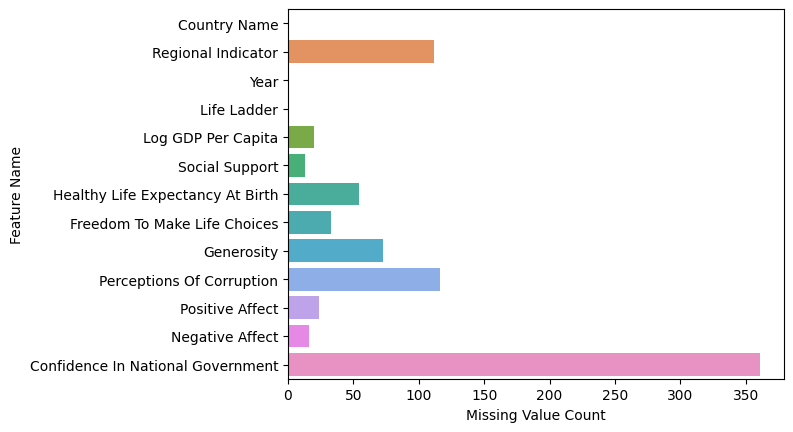
\includegraphics[width=15cm, height=10cm, keepaspectratio]{img/MissingValuesCount.png}       \caption{Displaying missing values count against each feature of dataset.}                  
\label{fig: Missing Values}
\end{figure}
\newpage

After the identification of null values, there are two ways to handle the missing values issue. First, we will drop all those values and the other one to fill those values with mean or median values if the column contains numeric data and mode when a column contains categorical data. In our case, we stuck to the first one and removed the missing values. Subsequently, the data set was checked for duplicate rows. However, The data did not contain any duplicate values. 

\subsection{Data Distribution}
we can see that this is a dataset based on World Happiness Report related to country-level happiness and various socioeconomic factors for the years 2005-2021. A few key observations are the sample contains 1,683 observations, likely representing different country-years. The mean year is around 2013, so this dataset covers nearly a 20 year span of time. Life Ladder is the target variable that ranges from 2.178809 to 7.970892 with a mean value of 5.484487 which indicates that happiness increases as the value of the Life Ladder variable increases. Log GDP per capita, a measure of economic prosperity, also demonstrates variation across the countries from min 5.52 to max 11.66. The six factors - social support, life expectancy, freedom, generosity, perceptions of corruption, and positive affect - have means in the 0.65 to 0.81 range on scales perhaps from 0 to 1, showing decent variation. Negative affect has a lower mean of 0.26, while confidence in government sits at 0.48 mean.

The standard deviations indicate there is dispersion from the means in all variables.
Overall, this summary suggests the data captures differences in subjective well-being and related economic and social factors across many countries over nearly 20 years. The breadth provides a solid foundation for analyzing how variables like GDP, social support, and governance correlate with and potentially influence happiness across nations and over time. The histogram shown in Figure \ref{fig: Life Ladder Histogram} shows that data has been distributed slightly lean towards higher values with the mean value of 5.48. Similarly, the data distribution among the other numeric features was also described in Table \ref{table:Data Distribution}.


\begin{figure}
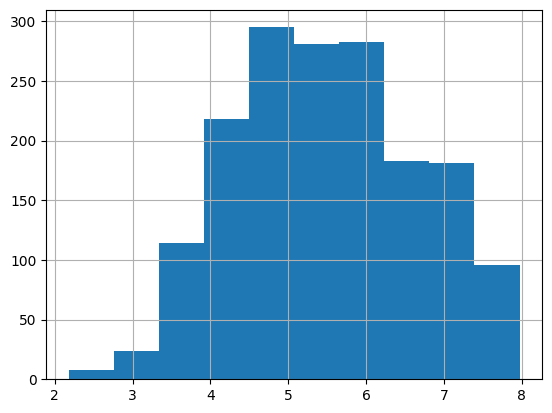
\includegraphics[width=15cm, height=10cm, keepaspectratio]
{img/LifeLadderHist.png}       
\caption{The histogram of the feature Life Ladder describes the data has been distributed among all values.}                  
\label{fig: Life Ladder Histogram}
\end{figure}
\newpage

\begin{table}[!htb]
\caption{Data Distribution.}
\begin{tabular}{|p{4.0cm}|c|c|c|c|c|c|c|c|c|}
\hline
Variable & count & mean & std & min & 25\% & 50\% & 75\% & max \\
\hline
Year & 1683 & 2013.92 & 4.4 & 2005 & 2010 & 2014 & 2018 & 2021 \\
\hline
Life Ladder & 1683 & 5.48 & 1.14 & 5.52 & 4.62 & 5.43 & 6.31 & 7.97 \\
\hline
Log GDP Per Capita & 1683 & 9.35 & 1.15 & 5.52 & 8.42 & 9.5 & 10.31 & 11.66 \\
\hline
Social Support & 1683 & 0.81 & 0.12 & 0.29 & 0.74 & 0.83 & 0.90 & 0.98 \\
\hline
Healthy Life Expectancy At Birth & 1683 & 63.1 & 7.1 & 6.7 & 58.4 & 65 & 68.9 & 74.3 \\
\hline
Freedom To Make Life Choices & 1683 & 0.74 & 0.13 & 0.26 & 0.65 & 0.76 & 0.85 & 0.98 \\
\hline
Generosity & 1683 & 0.0026 & 0.16 & -0.33 & -0.10 & -0.02 & 0.095 & 0.70 \\
\hline
Perceptions Of Corruption & 1683 & 0.75 & 0.18 & 0.035 & 0.69 & 0.80 & 0.87 & 0.98 \\
\hline
Positive Affect & 1683 & 0.65 & 0.10 & 0.17 & 0.57 & 0.67 & 0.74 & 0.88 \\
\hline
Negative Affect & 1683 & 0.26 & 0.081 & 0.094 & 0.2 & 0.25 & 0.31 & 0.6 \\
\hline
Confidence In National Government & 1683 & 0.48 & 0.19 & 0.07 & 0.33 & 0.46 & 0.61 & 0.99 \\
\hline
\end{tabular}
\label{table:Data Distribution}
\end{table}

\section{Data Analysis}
Countries with higher life ladder scores are represented on the map in dark green, while those with lower scores are shown in dark blue. You can view the life ladder scores for various years from 2005 to 2021 using the slider at the bottom of the map as shown in Figure \ref{fig: World  Happiness Map}
\begin{figure}[h!]
\centering
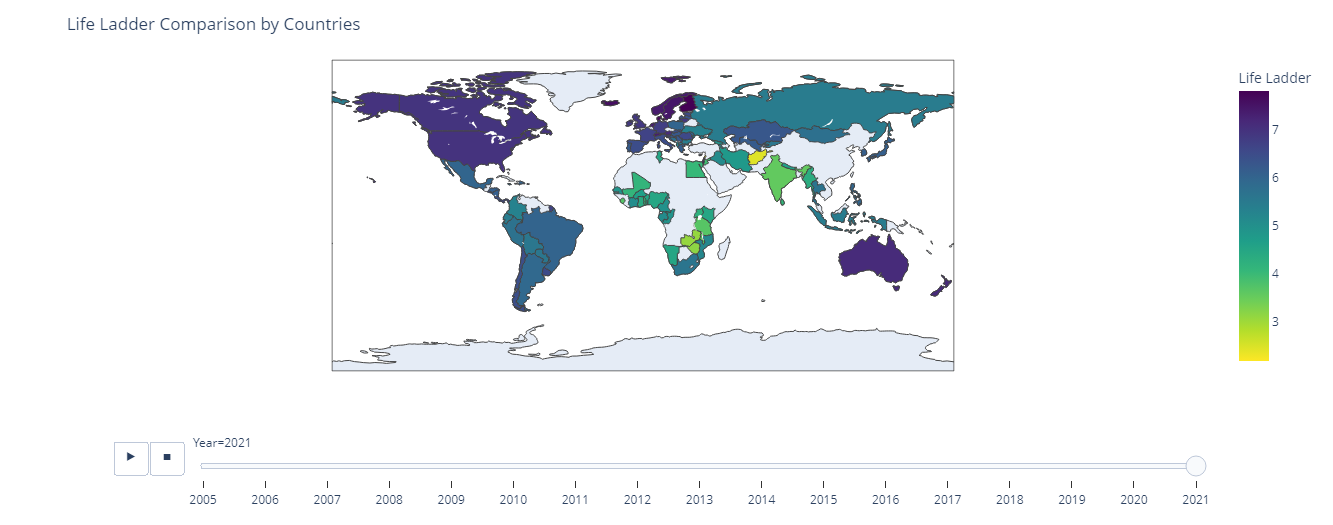
\includegraphics[width=15cm, height=10cm, keepaspectratio]{img/LifeLadderWW2021.png}       
\caption{World  Happiness Map.}                  
\label{fig: World  Happiness Map}
\end{figure}
\subsection{Most Happy Countries}
Denmark, Finland, Switzerland, Norway, and Netherlands were the  Happiest countries in 2022. Denmark is the Happiest country with a value of 7.66 followed by Finland, Switzerland, Norway, and Netherlands with a score of 7.61, 7.53, 7.5, and 7.46 respectively as shown in Figure \ref{fig: Top 5 Most Happiest countries}.
\begin{figure}[h!]
\centering
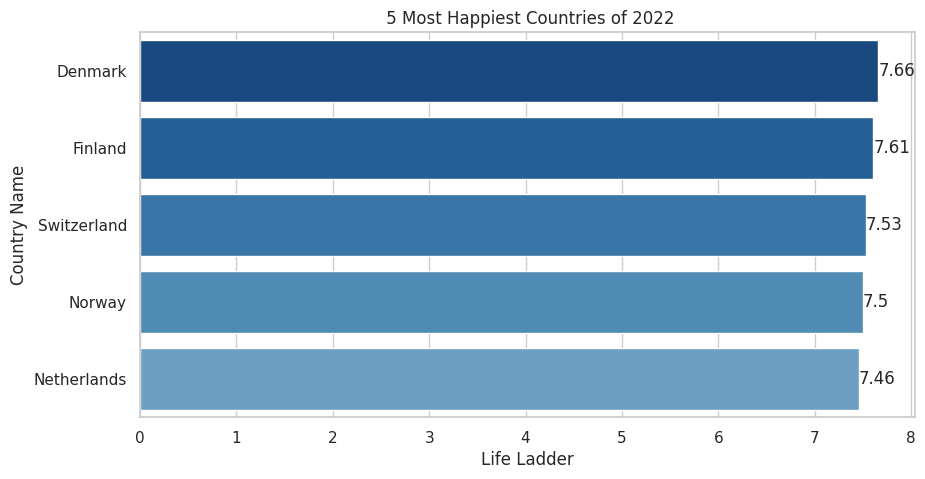
\includegraphics[width=15cm, height=15cm, keepaspectratio]{img/5MostHappiestCountries.png}       \caption{Top 5 Most Happy Countries.}                  
\label{fig: Top 5 Most Happiest countries}
\end{figure}

\subsection{Least Happy Countries}
Afghanistan, Togo, Rwanda, Burundi, and Tanzania were the Least happy countries. Afghanistan is the least happy country with a value of 3.51 in the perception of the corruption index. Togo, Rwanda, Burundi, and Tanzania are the least happy countries with index values of 3.6, 3.61, 3.69, and 3.7 respectively 

% as shown in Figure \ref{fig: Top 5 Least Happiest countries}.
% \begin{figure}[h!]
% \centering
% 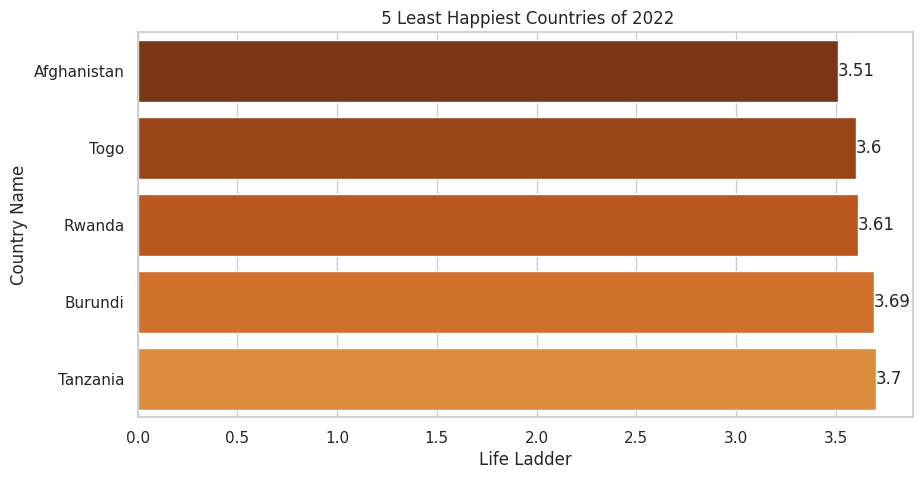
\includegraphics[width=15cm, height=15cm, keepaspectratio]{img/5LeastHappiestCountries.png}       \caption{Top 5 Least Happy Countries.}                  
% \label{fig: Top 5 Least Happiest countries}
% \end{figure}
% \newpage

\subsection{Most Corrupt Countries}
Romania, Bosnia, Bulgaria, Ukraine, and Moldova were the most corrupt countries for the year 2022. Romania is the most corrupt country with a value of 0.96 in the perception of the corruption index. Bosnia and Bulgaria shared the second spot in the perception of the corruption index with a value of 0.95 each. Similarly, Ukraine and Moldova shared the third spot in the perception of the corruption index with a value of 0.94 each as shown in Figure \ref{fig: Top 5 Most corrupt countries}.
\begin{figure}[h!]
\centering
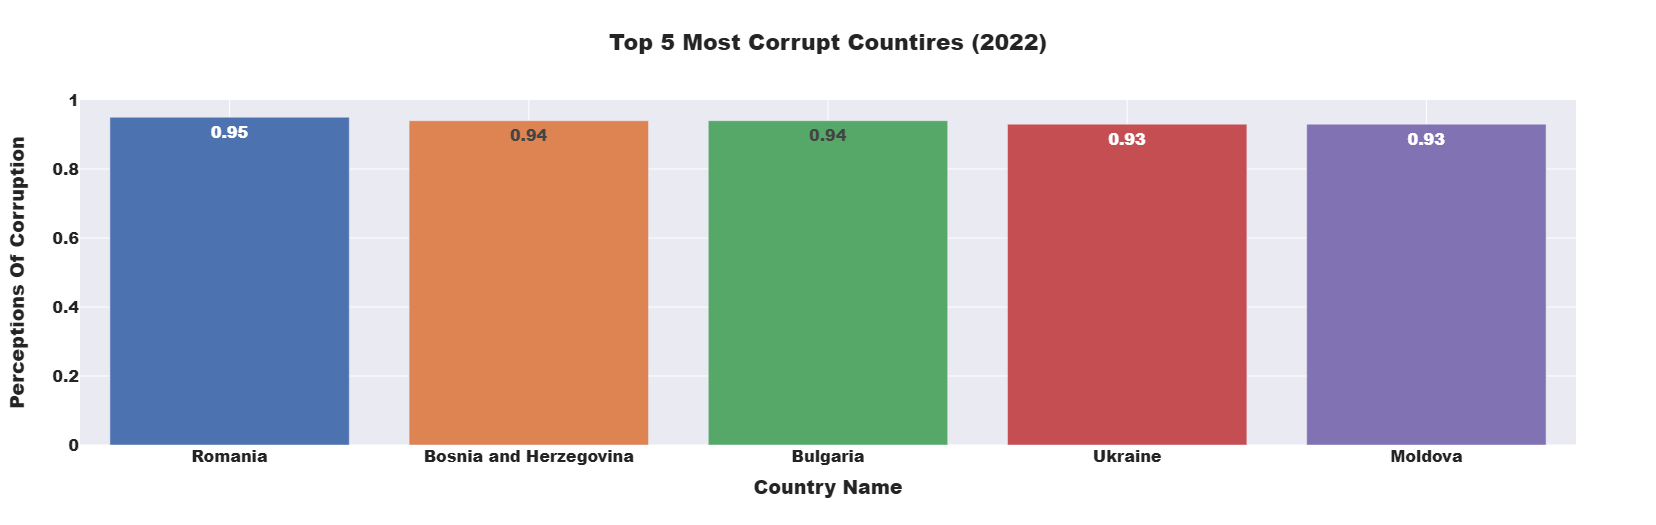
\includegraphics[width=18cm, height=10cm, ]{img/corrtop5.png}       \caption{Top 5 Corrupt Countries.}                  
\label{fig: Top 5 Most corrupt countries}
\end{figure}

\subsection{Least Corrupt Countries}
Singapore, Denmark, Rwanda, Finland, and Sweden were the Least corrupt countries in year 2022. Singapore is the Least corrupt country with a value of 0.1 in the perception of the corruption index. Denmark, Rwanda, Finland, and Sweden are the least corrupt countries with values of 0.2, 0.23, 0.24, and 0.26 in the perception of the corruption index respectively as shown in Figure \ref{fig: Top 5 Least corrupt countries}.
\begin{figure}[h!]
\centering
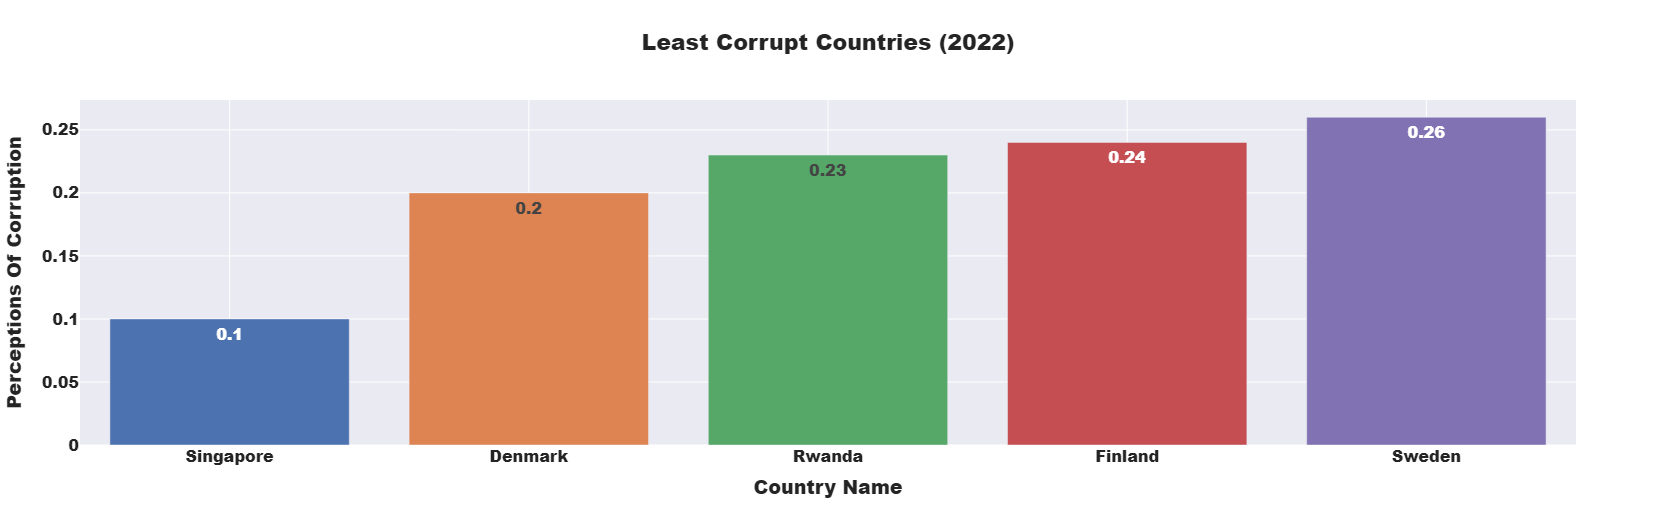
\includegraphics[width=18cm, height=10cm,]{img/corrlow5.png}       \caption{Least 5 Corrupt Countries.}                  
\label{fig: Top 5 Least corrupt countries}
\end{figure}
\newpage

\subsection{Most Social Countries}
In the list of most social countries of the world Iceland, Denmark, New Zealand, Ireland, and  Finland are ranked top five. They achieved rankings of 0.98, 0.96, 0.95, 0.95, and 0.95 respectively as shown in Figure \ref{fig: Top 5 Social countries}.
\begin{figure}[h!]
\centering
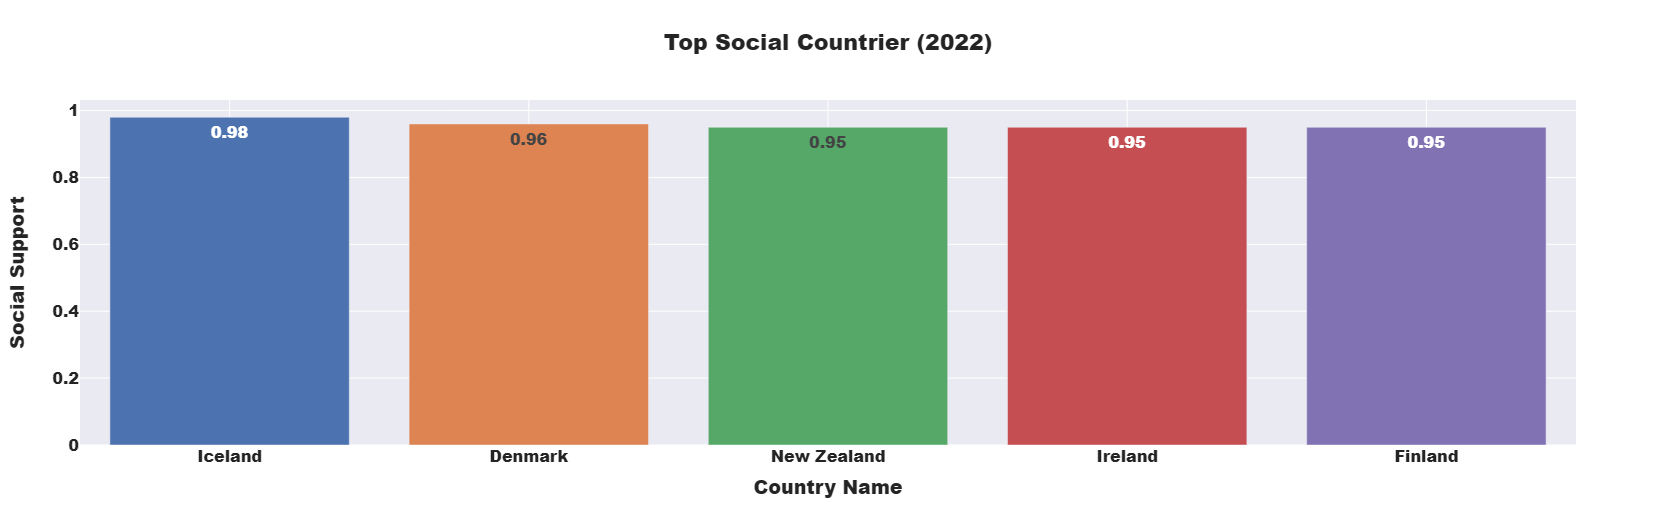
\includegraphics[width=16cm,height=10cm,]{img/sstop5.png}       \caption{Top 5 Social Countries.}                  
\label{fig: Top 5 Social countries}
\end{figure}
\newpage

\subsection{Least Social Countries}
Burundi, Togo, Benin, Afghanistan, and Rwanda are the least social countries in the world. They achieved rankings of 0.37, 0.47, 0.47, 0.5, and 0.56 respectively. Countries like Afghanistan and Burundi have faced years of war and civil unrest, disrupting social institutions and infrastructure as shown in Figure \ref{fig: Least 5 Social Countries}.
\begin{figure}[h!]
\centering
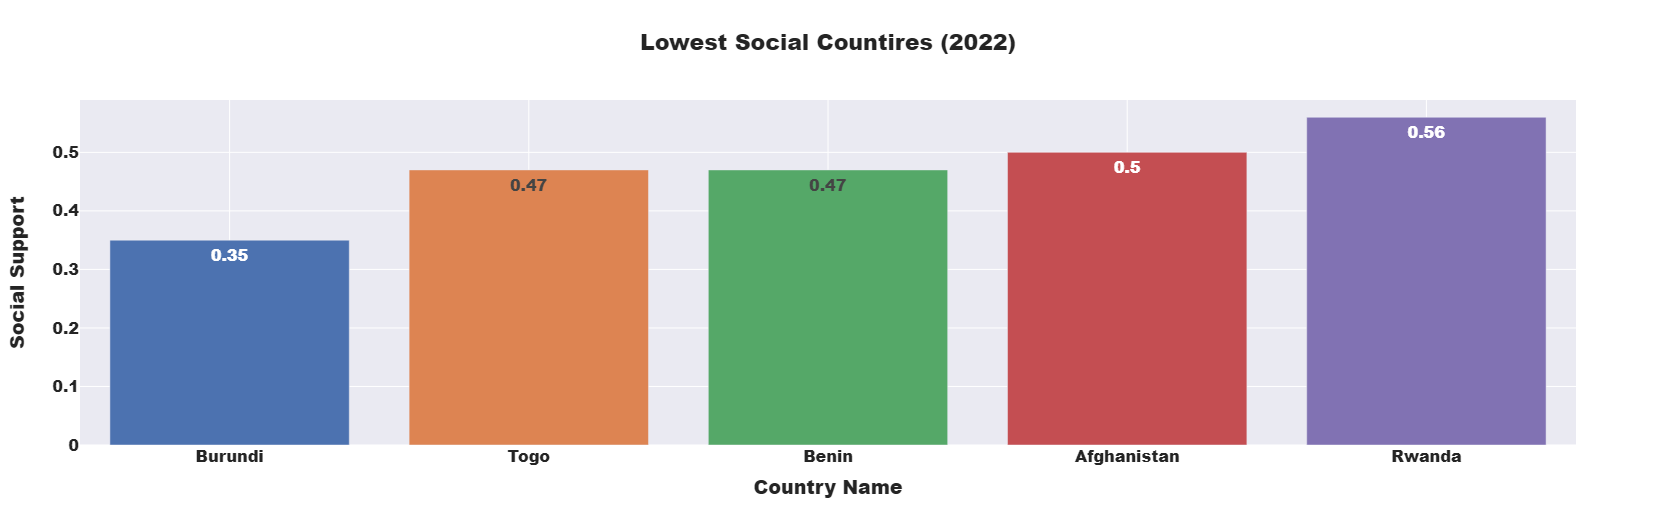
\includegraphics[width=18cm, height=10cm,]{img/sslow5.png}       \caption{Least 5 Social Countries.}                  
\label{fig: Least 5 Social Countries}
\end{figure}
\newpage

\subsection{Happiness among Region of the World}
North America and ANZ are the happiest regions of the world with a life ladder score of  7.24.  Western Europe stands second on the list with a score of 6.87. Latin America and Caribbean, East Asia, Central and Eastern Europe, Southeast Asia, Commonwealth of Independent States, and Middle East and North Africa stood 3, 4, 5, 6, 7, and 8 respectively on the happiness chart. South Asia and Sub-Saharan Africa were placed in the last two places in the chart of happiness among regions of the world as shown in Figure \ref{fig:RegionHappiness}.
\begin{figure}[h!]
\centering
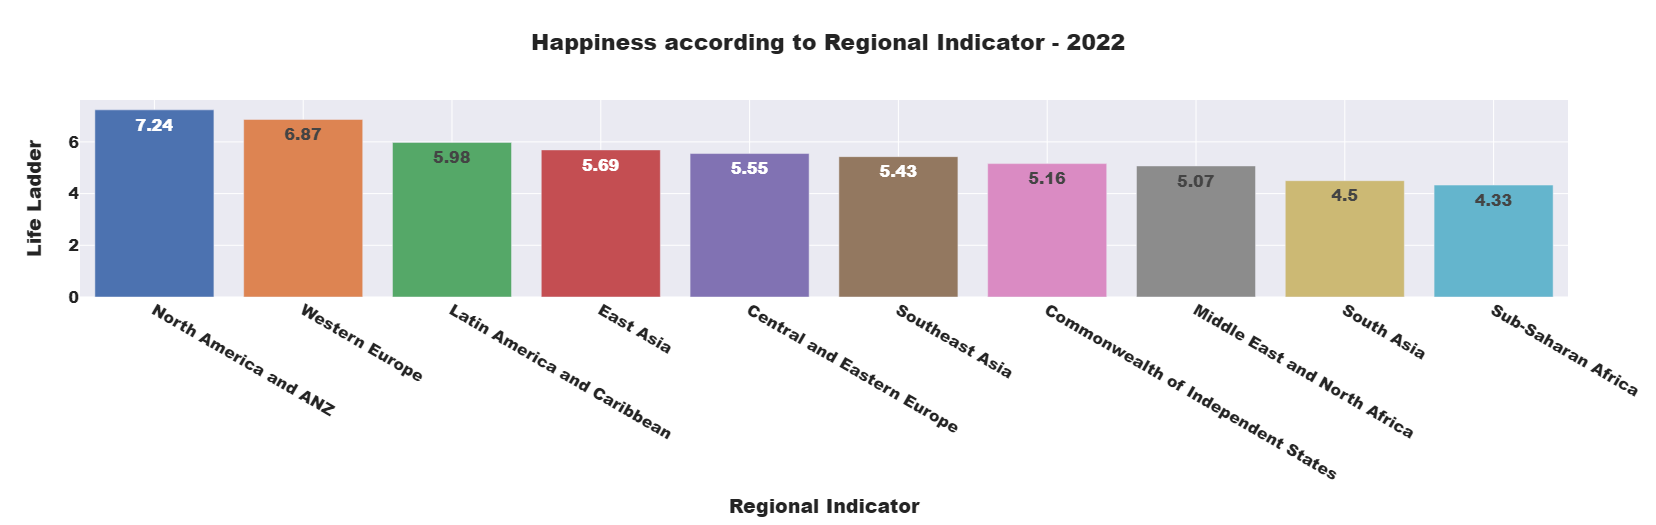
\includegraphics[width=15cm, height=8cm]{img/RegionHappiness.png}     
\caption{Happiness across various regions of the world.}                  
\label{fig:RegionHappiness}
\end{figure}
\newpage

\subsection{Social Support among regions of the World}
North America and ANZ are the social regions of the world with a social support score of  0.94.  Western Europe stands second on the list with a score of 0.92.  East Asia, Central and Eastern Europe, Latin America and Caribbean, Commonwealth of Independent States, Southeast Asia, and Middle East and North Africa stood 3, 4, 5, 6, 7, and 8 respectively on the happiness chart. Sub-Saharan Africa and South Asia were placed in the last two places in the chart of social support among regions of the world as shown in Figure \ref{fig:RegionSS}.
\begin{figure}[h!]
\centering
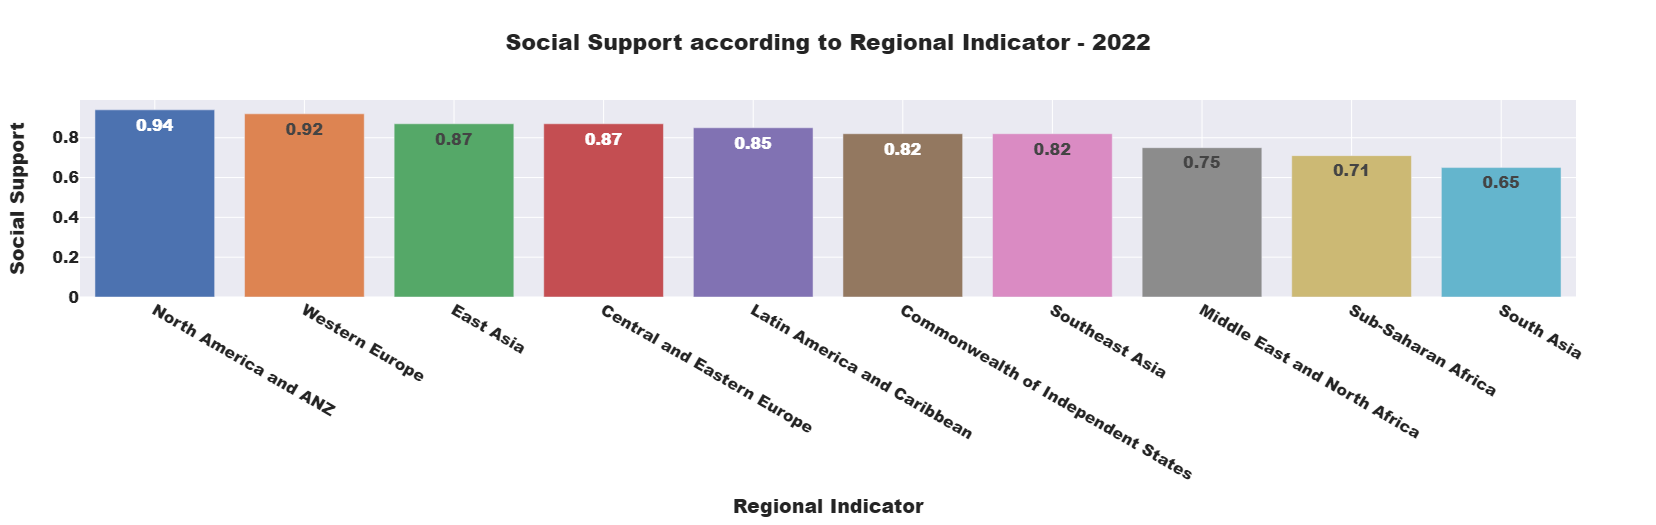
\includegraphics[width=15cm, height=8cm,]{img/RegionSS.png}     
\caption{Social Support across various regions of the world.}                  
\label{fig:RegionSS}
\end{figure}
\newpage

\subsection{Perception of corruption among Region of the World}
 Central and Eastern Europe are the most corrupt region of the world with a perception of corruption score of  0.87. Middle East and North Africa stands second on the list with a score of 0.82. South Asia, Sub-Saharan Africa, East Asia, Commonwealth of Independent States, Latin America and Caribbean, and Southeast Asia  stood 3, 4, 5, 6, 7, and 8 respectively on the happiness chart. North America and ANZ and Western Europe were placed in the last two places in the chart of corrupt regions of the world as shown in Figure \ref{fig:Region Perception of Corruption}.
\begin{figure}[h!]
\centering
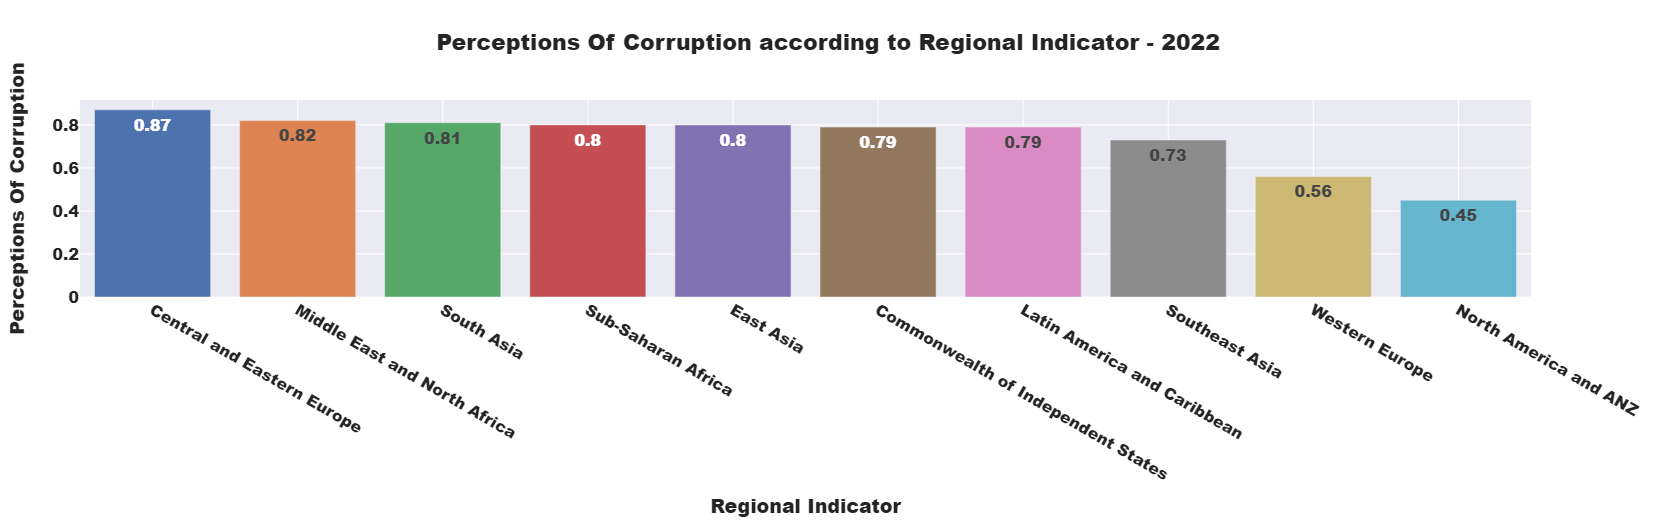
\includegraphics[width=15cm, height=8cm, ]{img/Region Perception of Corruption.png}     
\caption{Social Support across various regions of the world.}                  
\label{fig:Region Perception of Corruption}
\end{figure}
\newpage


\section{Feature Engineering:}
Conduct exploratory data analysis to gain insights into the relationships between happiness and other factors. The log of GDP per capita has a handsome positive relation with life ladder or other words happiness, Similarly, Social support and health life expectancy at birth also have a good positive relation with the life ladder with values of 0.72 and 0.74. On the other hand perception of corruption and negative affect have an inverse relation with life ladder as shown in Figure \ref{fig: Features Correlation}
\begin{figure}[h!]
\centering
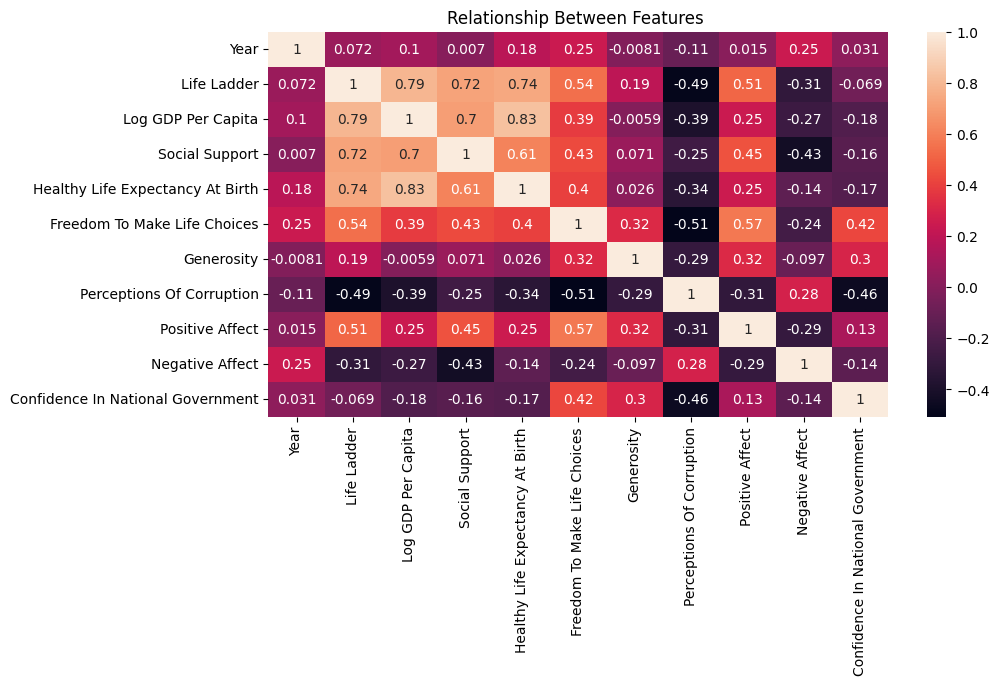
\includegraphics[width=15cm, height=15cm, ]{img/Correlation.png}       \caption{Features Correlation Map.}                  
\label{fig: Features Correlation}
\end{figure}
\newpage
Selected five relevant features based on T-Test analysis using Pearson\'s equation.\\

\begin{equation}
r = \frac{\sum\limits_{i=1}^{n} (x_i - \bar{x})(y_i - \bar{y})}{\sqrt{\sum\limits_{i=1}^{n} (x_i - \bar{x})^2} \sqrt{\sum\limits_{i=1}^{n} (y_i - \bar{y})^2}}
\end{equation}

\begin{equation}
t = r \sqrt{\frac{1 - r^2}{n - 2}}
\end{equation}
\subsection{Log per GDP capita}
One of Our Pearson Correlation Hypothesis for Log per GDP capita and life ladder is as follows:
\begin{itemize}
    \item Ho - Columns do not correlate
    \item Ha - Columns do Correlate
\end{itemize}

 \[statistic=0.7925\ \]
 \[P-value= 0.0  \] 
on the basis of the Pearson correlation coefficient valued 0.7925 between Log GDP per capita and Life Ladder, we can conclude that these two variables have a strong positive correlation that is statistically significant. The null hypothesis states that the two columns do not correlate. However, the Pearson coefficient of 0.7925 indicates a strong positive relationship - as one variable increases, the other tends to increase. Additionally, the p-value testing the significance of this correlation is 0.0, which is below the standard 0.05 threshold. This indicates we can reject the null hypothesis. The large positive Pearson coefficient and highly significant p-value provide clear evidence to reject the null hypothesis and conclude the Log GDP per capita and Life Ladder columns have a strong statistically significant positive correlation. The data shows as income increases, happiness levels also tend to rise across countries. This aligns with economic theories that higher GDP and income are linked to greater subjective well-being.
\subsection{Social Support}
Similarly, our second Pearson Correlation Hypothesis for Social Support and life ladder is as follows:
\begin{itemize}
    \item Ho - Columns do not correlate
    \item Ha - Columns do Correlate
\end{itemize}

 \[statistic=0.7206\ \]
 \[P-value= 1.1413\ e^{-269}  \]
According to the relatively strong positive correlation between Social Support and Life Ladder, which has a Pearson correlation coefficient of 0.7206, these two variables are statistically significant. According to the null hypothesis, the two columns do not correlate. The Pearson coefficient of 0.7206, on the other hand, suggests a positive link - when one variable increases, so does the other.

Moreover, the correlation's significance is tested using a p-value, which is 1.1413e-269, which is quite low. This is significantly lower than the typical 0.05 cutoff. This means that we can categorically reject the null hypothesis.The robust positive Pearson coefficient of 0.7206 and the unusually modest p-value give persuasive evidence to reject the null hypothesis. The Social Support and Life Ladder columns have a statistically significant relatively strong positive link, we can conclude. This implies that stronger social support is associated with greater pleasure across countries.

As a result, I agree with the conclusion that the null hypothesis should be rejected and that the two variables show a substantial positive connection. This is consistent with beliefs that larger social support networks promote greater subjective well-being and life satisfaction as mentioned in Figure \ref{fig: Features Correlation}

\subsection{Perceptions Of Corruption} 
Another, Pearson Correlation Hypothesis for Perceptions Of Corruption and the life ladder is as follows:
\begin{itemize}
    \item Ho - Columns do not correlate
    \item Ha - Columns do Correlate
\end{itemize}
, 
 \[statistic = -0.4921633408644486\ \]
 \[P-value = 2.2381 e^{-103}  \]
With a Pearson correlation coefficient of -0.49216 between Perceptions of Corruption and Life Ladder, we can conclude that these two variables have a moderately negative and statistically significant link. According to the null hypothesis, the columns do not correlate. The Pearson coefficient of -0.49216, on the other hand, implies an inverse relationship: when one variable increases, the other tends to decrease.


Furthermore, the p-value for assessing this correlation is exceedingly low at 2.2381e-103. This is considerably below the 0.05 significance level, allowing us to reject the null hypothesis with confidence. The minuscule p-value combined with the negative Pearson coefficient of -0.49216 gives strong evidence against the null hypothesis. The Perceptions of Corruption and Life Ladder columns have a statistically significant moderate negative association, we can conclude. This shows that higher levels of corruption are connected with lower levels of happiness across countries. Happiness tends to decline when perceived corruption rises. As a result, I agree that the null hypothesis should be rejected based on the facts. This is consistent with assumptions that views of honesty and transparency in government and institutions are associated with higher levels of well-being.

\subsection{Healthy Life Expectancy At Birth}
Another, Pearson Correlation Hypothesis for Healthy Life Expectancy At Birth and the life ladder is as follows:
\begin{itemize}
    \item Ho - Columns do not correlate
    \item Ha - Columns do Correlate
\end{itemize}
, 
 \[statistic = 0.7351608503079882\ \]
 \[P-value = 4.018539154290545 e^{-286}  \]
Healthy Life Expectancy at Birth and Life Ladder have a strong positive link that is statistically significant, according to the Pearson correlation value of 0.73516. The columns are not correlated, according to the null hypothesis. The Pearson coefficient of 0.73516, however, shows a strong positive correlation, meaning that as one variable rises, the other generally tends to rise as well. Additionally, the p-value used to assess this correlation is quite low at 4.0185e-286. The null hypothesis can be categorically rejected because this is significantly below the threshold of 0.05.

The minuscule p-value and the enormous positive Pearson coefficient of 0.73516 give strong evidence against the null hypothesis. We can state unequivocally that there is a statistically significant strong positive link between the Life Ladder and Healthy Life Expectancy at Birth columns. This means that greater levels of happiness are found in all countries where life expectancies are higher. Happiness scores improve along with life expectancy. I concur that the statistically significant strong positive correlation shown in the data should lead us to reject the null hypothesis. This supports the hypothesis that strong relationships exist between subjective well-being and lifespan as well as excellent health.


\subsection{Freedom To Make Life Choices}
Another, Pearson Correlation Hypothesis for Freedom To Make Life Choices and the life ladder is as follows:
\begin{itemize}
    \item Ho - Columns do not correlate
    \item Ha - Columns do Correlate
\end{itemize}
, 
 \[statistic = 0.5422970891885058\ \]
 \[P-value = 2.691858106607973 e^{-129}  \]
With a relatively positive correlation between Freedom to Make Life Choices and Life Ladder and a statistically significant Pearson correlation coefficient of 0.54229, we can conclude that these two variables are related. The columns are not correlated, according to the null hypothesis. The Pearson coefficient of 0.54229, however, shows a positive association, meaning that as one variable rises, the other likely to rise as well.

As a result, the correlation's p-value is incredibly low, 2.6919e-129. This is far less than the threshold of 0.05, allowing us to categorically reject the null hypothesis. The small p-value and the positive Pearson coefficient of 0.54229 give significant evidence against the null hypothesis. We can state categorically that there is a statistically significant moderate positive link between the Freedom to Make Life Choices and Life Ladder columns. This shows that beyond national boundaries, greater freedom and autonomy are linked to higher levels of happiness. Happiness scores climb along with perceived freedom. Therefore, I concur that the statistically significant positive correlation shown in the data should lead us to reject the null hypothesis. This fits assumptions that subjective well-being is closely related to one's level of life agency.


\subsection{Data Splitting}
After that, we split the dataset into training and testing sets to evaluate model performance. the training set contains 70\% of the records while the test set contains 30\% of the whole dataset records.

In the end, We made three classes 'Happy', and 'Unhappy' based on our target variable which is numeric as shown in Figure \ref{fig: HappinessDistribution}
\begin{figure}[h!]
\centering
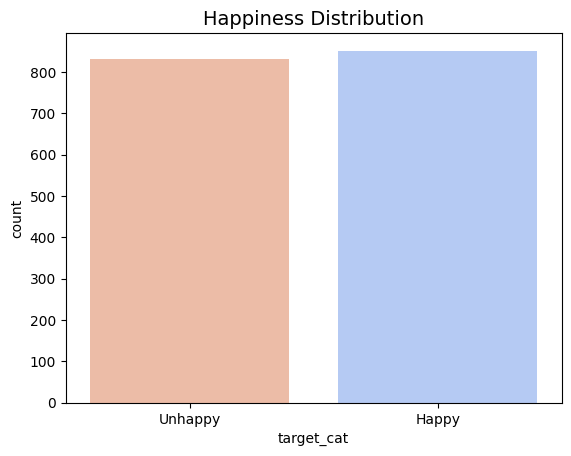
\includegraphics[width=15cm, height=15cm, keepaspectratio]{img/HappinessDistribution.png}       \caption{Happiness Variable Distribution.}                  
\label{fig: HappinessDistribution}
\end{figure}
\newpage
Subsequently, we applied a MinMaxScaler transformation on training and test features.


\section{Model Selection}

    
\subsection{Regression Model}
Logistic regression is a statistical technique used to predict binary outcomes based on historical data. It models the probability of an event, such as pass/fail, win/lose, alive/dead, etc.
The logistic regression formula is shown in the equation.
\begin{equation}
P(Y=1) = \frac{1}{1+e^{-(b_0 + b_1X_1 + b_2X_2 + ... + b_nX_n)}}
\end{equation}
\begin{itemize}
    \item P(Y=1) is the probability of the event occurring (coded as 1)
    \item e is the base of natural logarithms
    \item b0 is the intercept
    \item b1, b2...bn are the regression coefficients
    \item X1, X2...Xn are the predictor variables
\end{itemize}
For example, to predict if a student will pass an exam based on hours studied and previous GPA, the logistic regression equation would be:

\begin{equation}
P(\text{Pass exam}) = \frac{1}{1 + e^{-\ (b_0\ +\ b_1 \ times \ (\text{Study hours})\ +\ b_2  \ times \ (\text{GPA})}}.
\end{equation}

The coefficients b1 and b2 are estimated using maximum likelihood to best fit the logistic model with the data. This allows predicting the probability of passing for given study hours and GPA.

\subsection{Decision Tree}
A decision tree is a type of flowchart that has a series of internal nodes, each of which has a rule, and branches that show the results of the rules. The goal is to build a tree that maximizes information gain at each split. For classification, this means reducing the entropy in the child nodes.
Each internal node represents a test or decision on an attribute. Branches coming out of the node represent the outcomes of the test while leaf nodes at the end represent the final class label or predicted value for regression

Gini impurity is the primary parameter used to choose the optimum rule at a particular node. For a set of elements with N classes, the gini impurity is determined by equation as follows:

\begin{equation}
Gini = \sum_{i=1}^{N} p_i * (1 - p_i)
\end{equation}

Trees can capture nonlinear relationships and feature interactions. Some advantages of decision trees include interpretability, the ability to handle categorical variables, and requiring little data preprocessing. Limitations include overfitting and instability.
\subsection{Random Forest}
An approach used in machine learning that is based on grouping of multiple trees outcomes to merge in a single outcome  is known as random forest. The method used to resolve both classification issues and problems related to regression. In order to resolve the classification problem this technique collects estimated results from all learners and the converge to a single outcome based on majority voting. However, during regression anomalies it takes mean or average of all predicted results produced by learners or decision trees. The method first construct multiple decision trees then each tree is trained on training sample in order to make prediction on test data. After collecting the outcomes from each tree it consolidate the result to make one final prediction by using either mean or majority vote based on type of anomaly. There are some key characteristics of random forest described as follows.

\subsubsection{Ensemble of decision trees} The model have a group of decision trees trained using various random training sub samples of actual dataset used 
 for training.
\subsubsection{Bagging} Each tree is trained on a bootstrapped sample containing a random subset of data points from the original training set. This introduces variation which decreases the variance of the model.
\subsubsection{Random subsets of features} Each tree is built by picking a random subset of features to consider for splits at each node. This decorrelates the trees while still maintaining strength.
\subsubsection{Averaging outputs} The aggregate prediction of the decision trees are play its role to avoid the isssue of over fitting than individual  trees. For classification, majority vote of tree outputs is taken. For regression, the mean is calculated.\\

Random forest achieves high accuracy due to ensemble and decorrelated trees.
and avoids overfitting as compared to single decision tree. It can handle nonlinear relationships and high dimensional data and has embedded feature selection through random subsets. On the other hand it is prone to overfitting with noisy/sparse data.and can be slow to train and predict due to multiple trees.
\subsection{K Nearest Neighbour}
The K-Nearest Neighbors algorithm is a simple, supervised machine learning method used for both classification and regression tasks. It relies on measuring similarity between data points to make predictions. Some key characteristics of KNN is as discussed.

\subsubsection{Non-parametric} KNN does not make any assumptions about the underlying data distribution. It is also called lazy learning as it does not learn a model during training.
\subsubsection{Distance metrics} Distance functions like Euclidean described in equation \ref{eq:Euclidean}, Manhattan described in equation \ref{eq:Manhattan}, and Minkowski described in equation \ref{eq:Minkowski} distance are used to measure the proximity between data points. The closest k points are considered the neighbors. The equations of distance functions are as follows:\\
\subsubsection{Euclidean Distance:}
\begin{equation}
\label{eq:Euclidean}
d_{Euclidean}(\mathbf{x}, \mathbf{y}) = \sqrt{\sum_{i=1}^{n}(x_i - y_i)^2}
\end{equation}

\subsubsection{Manhattan Distance:}

\begin{equation}
\label{eq:Manhattan}
d_{Manhattan}(\mathbf{x}, \mathbf{y}) = \sum_{i=1}^{n}|x_i - y_i|
\end{equation}

\subsubsection{Minkowski Distance:}

\begin{equation}
\label{eq:Minkowski}
d_{Minkowski}(\mathbf{x}, \mathbf{y}) = \left(\sum_{i=1}^{n}|x_i - y_i|^{p}\right)^{\frac{1}{p}}
\end{equation}

Where $\mathbf{x}$ and $\mathbf{y}$ are two data points
$n$ is the number of dimensions
$p$ is the order of the Minkowski distance

\subsubsection{Majority voting} For classification, the class label of a data point is predicted by a majority vote of its k nearest neighbors in the training set.
\subsubsection{Averaging} For regression, the output is calculated by averaging the values of k nearest neighbors.
Parameter k - The model hyperparameter k determines how many neighbors to consider for the predictions. KNN is simple and easy to implement with low computational complexity and is effective for nonlinear separation boundaries and multiclass problems. It is robust to noisy data points since the algorithm averages neighbors. On the contrary, KNN's prediction cost is high for large datasets as the distance to all points must be calculated. It requires determining the optimal k parameter and distance metric for a problem
and performance degrades with high dimensional data due to distance measures.

\subsection{Support Vector Machine}
It is an other supervised learning approach works well in resolution of classifying issues as well as  problems related to regression.It operate in such a way that if an issue is not clearly segregating the various classes in two dimension space the it introduce more dimension in order to resolve the problem.  The objective is to search a hyper plane that clearly separates the different classes with maximum margin. the major characteristics consist of following.

\subsubsection{Maximal marginal hyperplane} SVM finds the optimal hyperplane with maximum margin between classes by maximizing the distance between closest points of different classes (support vectors).
\subsubsection{Kernel function} SVMs use kernel functions like polynomial or RBF to transform data into higher dimensions where it may become linearly separable. This allows modeling complex nonlinear decision boundaries.
\subsubsection{Regularization} SVM utilizes regularization parameters to prevent overfitting and allow some misclassifications. This improves robustness on unseen data.\\


SVMs solve a quadratic optimization problem to find optimal parameters that maximimize the margin. For non-linearly separable data, soft margin SVM provides slack variables to allow some misclassifications. The dual Lagrangian form, solved via quadratic programming, provides efficient training.It is effective for high dimensional spaces and clear margins between classes and memory efficient as support vectors fully represent the model. SVM is versatile due to the use of kernel functions for nonlinearity and is robust against overfitting through regularization. SVM is prone to overfitting and inefficient for non-linear boundaries with kernel trick. In SVM, choosing the right kernel function can be difficult. SVM is less interpretable compared to other techniques.


\section{Evaluation Metrics}
Evaluation metrics quantify the effectiveness of a classification model on a test dataset. The main categories are:

Here is the LaTeX code to format the classification performance metrics overview:

\begin{enumerate}

\item Accuracy-based metrics

\begin{itemize}

\item Accuracy: 
Accuracy is a common performance metric used to evaluate the performance of classification models, such as machine learning algorithms or classifiers. It measures the proportion of correctly predicted instances out of the total instances in the dataset. In other words, accuracy indicates how well the model is able to classify instances into their correct classes.
\begin{equation}
\label{eq:Accuracy}
Accuracy = \frac{Number\ of\ correct\ predictions}{Total\ number\ of\ predictions}
\end{equation}
\end{itemize}
Suppose you have a dataset of emails, and you're building a spam filter. Each email is labeled as either "spam" or "not spam". You train your model using this data and then test it on a separate set of emails. There are 200 emails in the test set and 150 emails are correctly classified as "not spam" while 30 emails are correctly classified as "spam". The number of correct predictions is 180 and the total number of predictions is 200. This means that your spam filter model correctly predicted the class of 90\% of the emails in the test set.

\item Confusion matrix-based metrics

\begin{itemize}
\item Precision: The proportion of cases that are truly positive among those that were expected to be positive is measured by precision, a performance indicator used in classification tasks. In other words, it counts the number of cases that really fall into the positive category among those that were expected to be positive.

We have a dataset with 100 emails, out of which 20 are spam and 80 are not spam. Our classifier predicts that 25 emails are spam, out of which 15 are actually spam and 10 are not spam. In this case, the precision of our classifier is calculated as the number of true positives (15) divided by the total number of instances predicted as positive (25), which gives us a precision of 0.6. Precision is an important metric in situations where false positives are more costly than false negatives. For example, in a medical diagnosis scenario, it is more important to correctly identify patients who have a disease (true positives) than to incorrectly identify healthy patients as having the disease (false positives).

\begin{equation}
\label{eq:Precision}
Precision = \frac{True:Positives}{True:Positives + False:Positives}
\end{equation}

\item Recall: Recall referred to as sensitivity or the true positive rate, is a performance indicator used in classification tasks to assess a model's capacity to properly identify all pertinent instances. Simply put, it informs us of the percentage of real positives that our model accurately identified.

Taking the above case, the recall of our classifier is calculated as the number of true positives (10) divided by the total number of actual positives (20), which gives us a recall of 0.5. Recall is an important metric in situations where false negatives are more costly than false positives. For example, in a medical diagnosis scenario, it is more important to correctly identify all patients who have a disease (true positives) than to miss some patients who have the disease (false negatives).



\begin{equation}
\label{eq:Recall}
Recall = \frac{True\ Positives}{True\ Positives + False\ Negatives}
\end{equation}

\item F1-score: 
The F1 score is a performance metric used in classification tasks to measure the balance between precision and recall. It is the harmonic mean of precision and recall. Suppose we have a binary classification problem where we want to predict whether an email is spam or not spam. 
We have a dataset with 100 emails, out of which 20 are spam and 80 are not spam. Our classifier predicts that 25 emails are spam, out of which 15 are actually spam and 10 are not spam. In this case, the precision of our classifier is calculated as the number of true positives (15) divided by the total number of instances predicted as positive (25), which gives us a precision of 0.6.  The recall of our classifier is calculated as the number of true positives (15) divided by the total number of actual positives (20), which gives us a recall of 0.75. The F1 score is then calculated as 2 * (0.6 * 0.75) / (0.6 + 0.75), which gives us an F1 score of 0.67.
The F1 score is an important metric in situations where both precision and recall are important, and we want to balance the trade-off between them. For example, in a medical diagnosis scenario, it is important to correctly identify patients who have a disease (true positives) while minimizing the number of healthy patients incorrectly identified as having the disease (false positives) and minimizing the number of patients who have the disease but are missed by the classifier (false negatives).

According to the given  example 
\end{itemize}
\begin{equation}
\label{eq:F1score}
F_1 Score = 2\ times\ \frac{PrecisionRecall}{Precision + Recall}
\end{equation}

\item Decision threshold metrics

\begin{itemize}
\item Auc-ROC: 
It is a performance metric utilized in classification tasks to measure the ability of a model to distinguish between positive and negative classes1. AUC is stands for area under the curve while ROC represents receiver operating curve. The ROC curve is  the graphical representation of both true and false positive rate for various values of threshold.In the graph x-axis is used false positive rate against the true positive rate on y-axis. 

The AUC is the representation of the probability that a classifier will rank a randomly chosen positive instance higher than a randomly chosen negative one. The values of AUC varies from 0 to 1, where an AUC value of 0 means that the model made 100\% wrong predictions, and 1 means that the model made 100\% wrong predictions.
Suppose we have a binary classification problem where we want to classify our emails into two classes either it is a spam mail or a regular mail.
We have a dataset with 100 emails, out of which 20 are spam and 80 are not spam.Our classifier predicts probabilities for each email being spam, and we can vary the threshold for classifying an email as spam or not spam.
By varying the threshold, we can calculate the TPR and FPR for each threshold setting, and plot these values to create the ROC curve. Once an ROC curve is plotted  all the area comes under the curve is known as area under the curve denoted as AUC.

AUC-ROC is useful in evaluating the performance of binary classifiers, as it provides a measure of how good the classifier is making prediction  in order to segregate the both classes. AUC-ROC is a scale-invariant method as it make same prediction either you use scaling of the features or not. Moreover, it is also invariant to classification threshold, mean that predictions is not effected by any value of threshold of classification or any change is made in threshold.

\item PRC: Precision-recall curve

PRC stands for Precision-Recall Curve, which is a performance metric used in classification tasks to measure the trade-off between precision and recall1. Recall is the percentage of relevant cases that were really fetched, whereas precision is the percentage of relevant occurrences among the obtained cases.


Suppose we have a binary classification problem where we want to predict whether an email is spam or not spam.
We have a dataset with 100 emails, out of which 20 are spam and 80 are not spam.
Our classifier predicts probabilities for each email being spam, and we can vary the threshold for classifying an email as spam or not spam.
By varying the threshold, we can calculate the precision and recall for each threshold setting, and plot these values to create the PRC.
The PRC is useful in evaluating the performance of binary classifiers, as it provides a visual representation of how well the model can distinguish between positive and negative classes at different threshold settings. It is particularly useful in imbalanced data sets, where one class is much more frequent than the other.

\end{itemize}
\newpage
\section{Code Flow Diagram}
In the study, Google co-lab is used as development environment with Python as the coding language. The version of python that is used is 10.0.4. During the coding various libraries has been used for different purposes that include data handling, mathematical calculations, visualisation and model training. The main libraries used in the development of the project are pandas, numpy, matplolib, seaborn and sklearn libraries. In the next step, Data has been loaded from the publically available link at https://www.kaggle.com/datasets/usamabuttar/world-happiness-report-2005-present. Then, we trained and tested the model and obtained results based on performance metrics. 

\begin{figure}
    \centering
    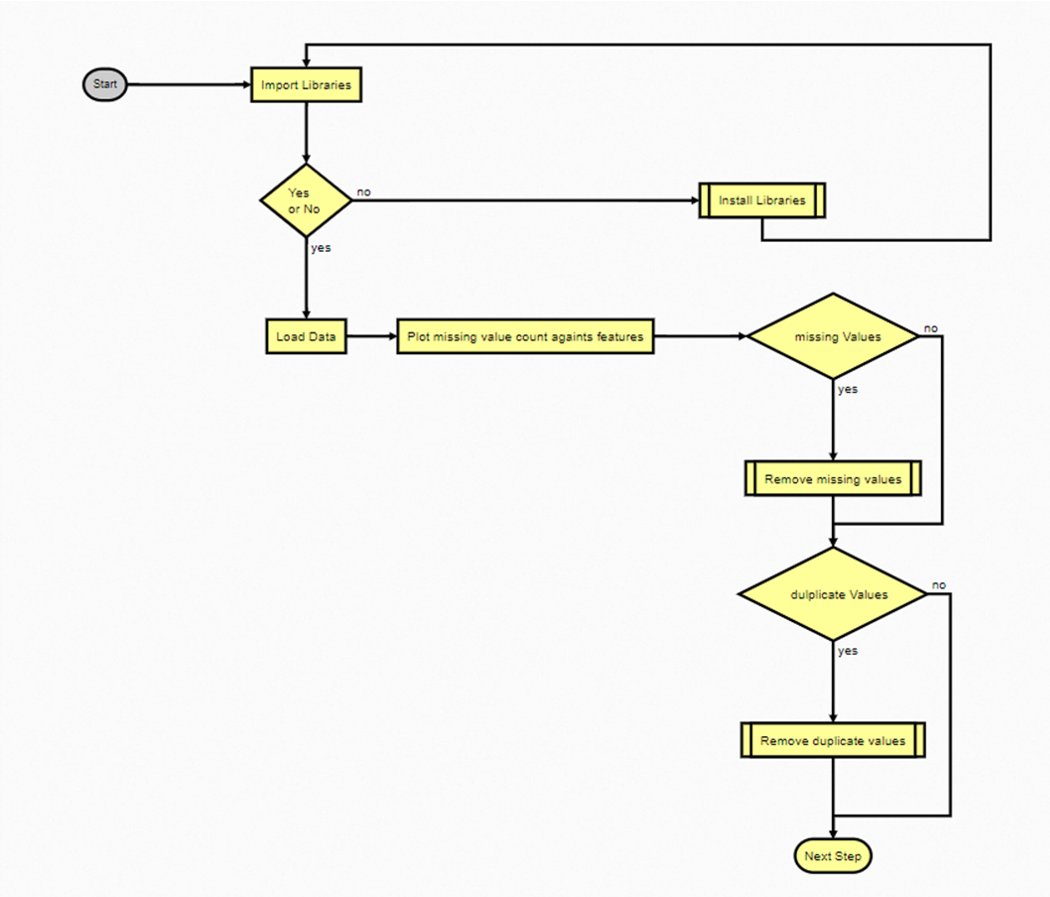
\includegraphics[width=15cm,height=15cm,keepaspectratio]{img/CodeFlow1.png}
    \caption{Code Flow diagram part 1}
    \label{fig:CodeFlow1}
\end{figure}
\begin{figure}
    \centering
    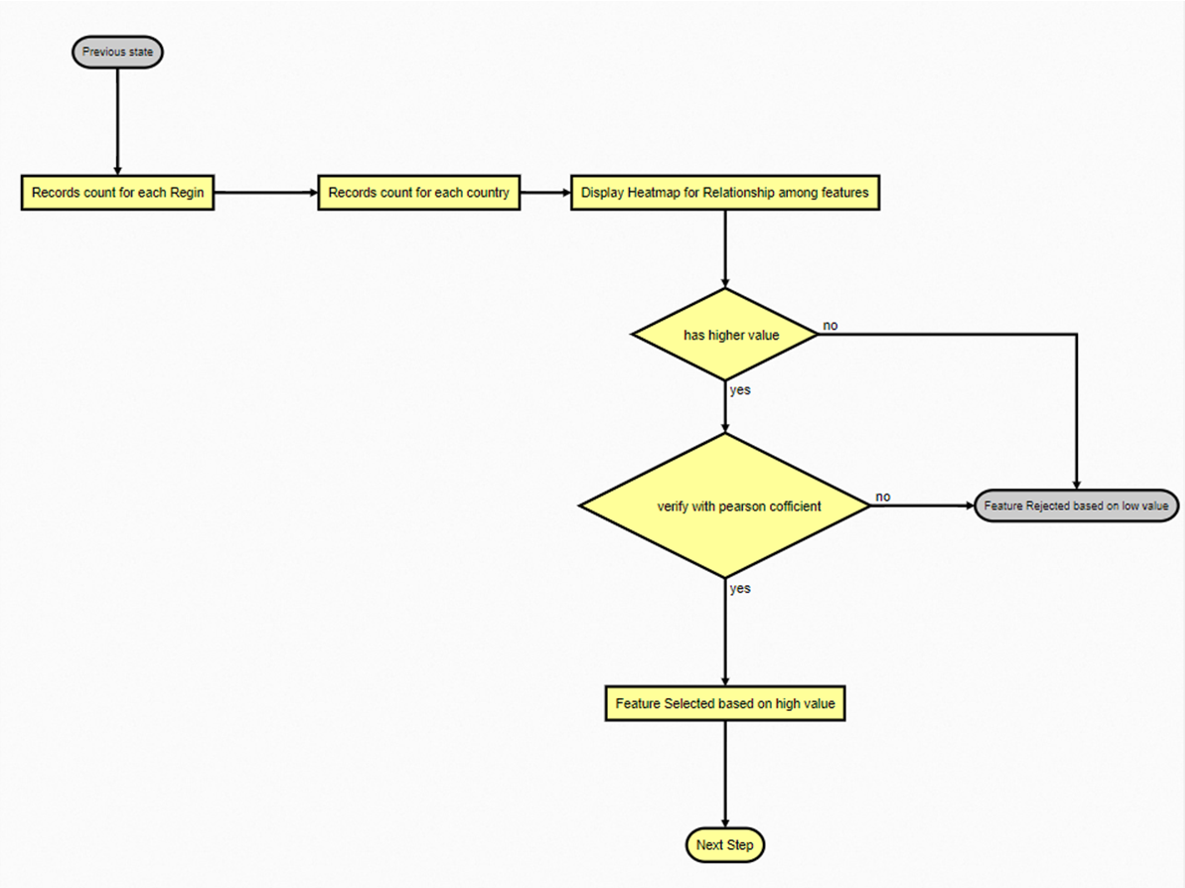
\includegraphics[width=15cm,height=15cm,keepaspectratio]{img/CodeFlow2.png}
    \caption{Code Flow diagram part 2}
    \label{fig:CodeFlow2}
\end{figure}
\begin{figure}
    \centering
    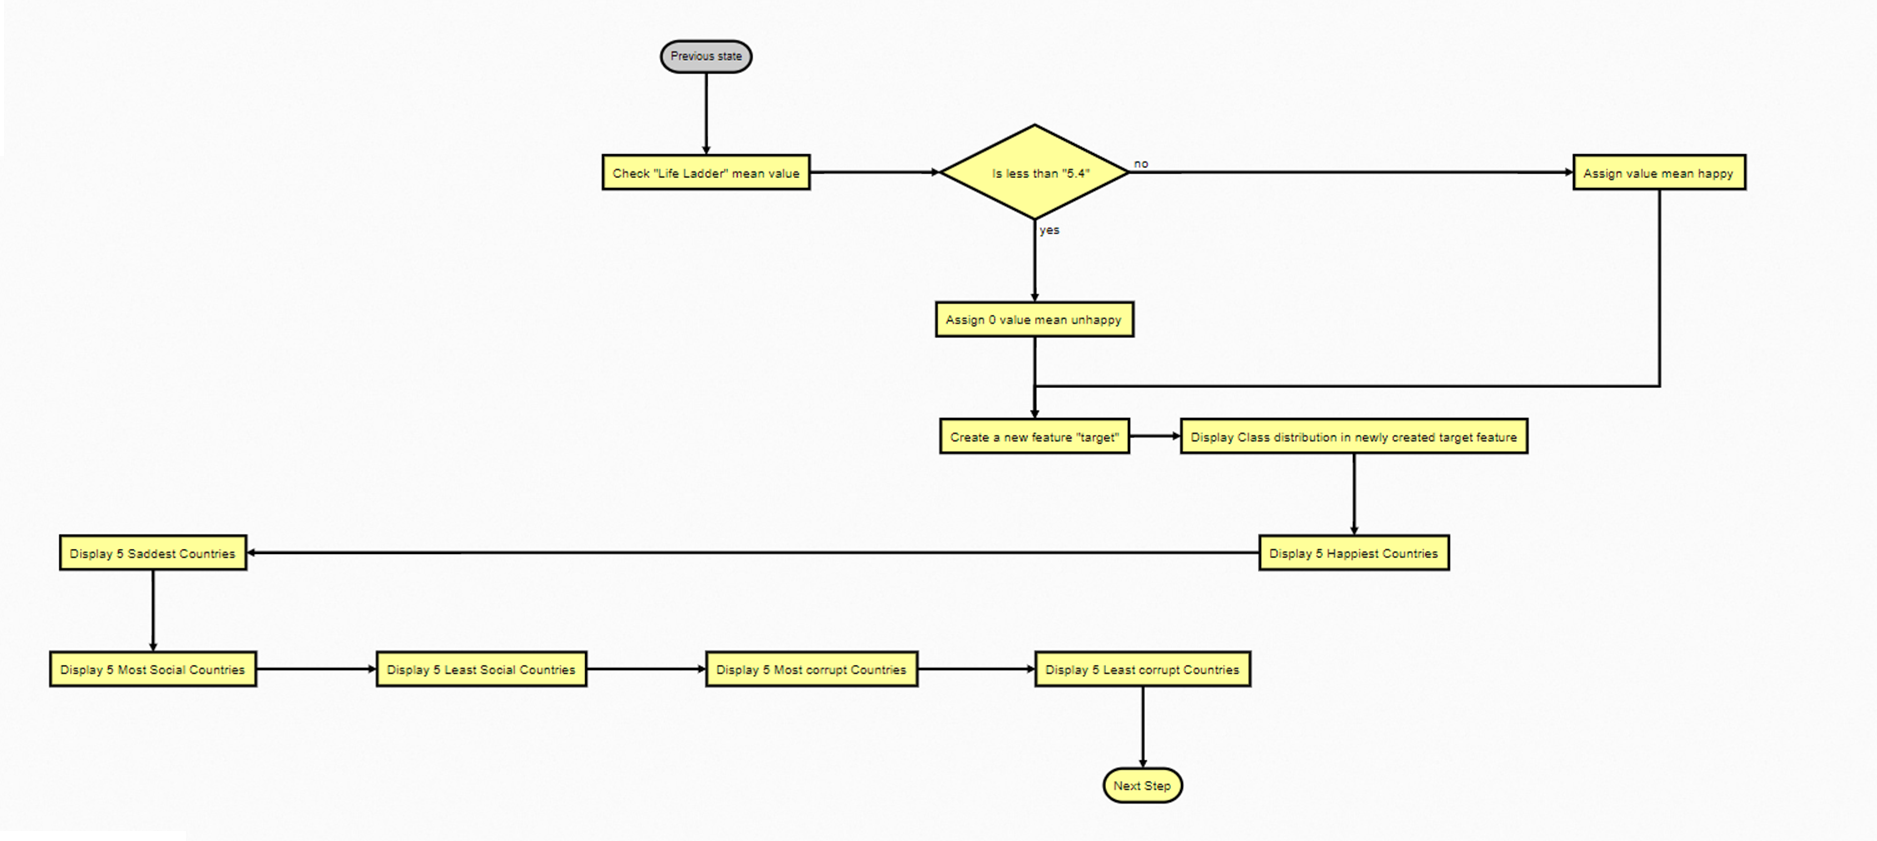
\includegraphics[width=15cm,height=15cm,keepaspectratio]{img/CodeFlow3.png}
    \caption{Code Flow diagram part 3}
    \label{fig:CodeFlow3}
\end{figure}
\begin{figure}
    \centering
    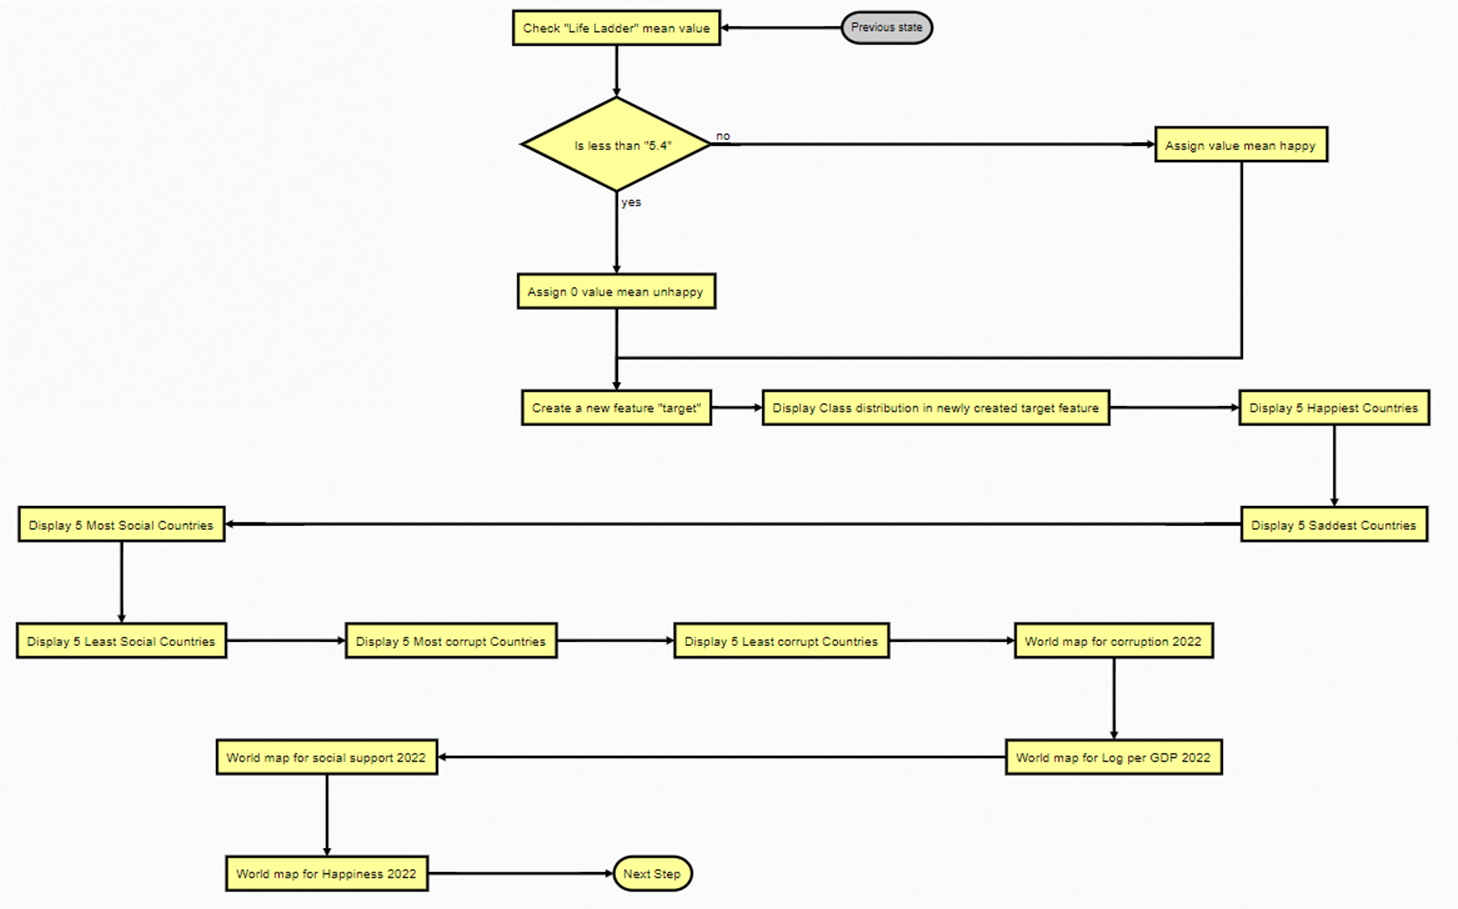
\includegraphics[width=15cm,height=15cm,keepaspectratio]{img/CodeFlow4.png}
    \caption{Code Flow diagram part 4}
    \label{fig:CodeFlow4}
\end{figure}
\begin{figure}
    \centering
    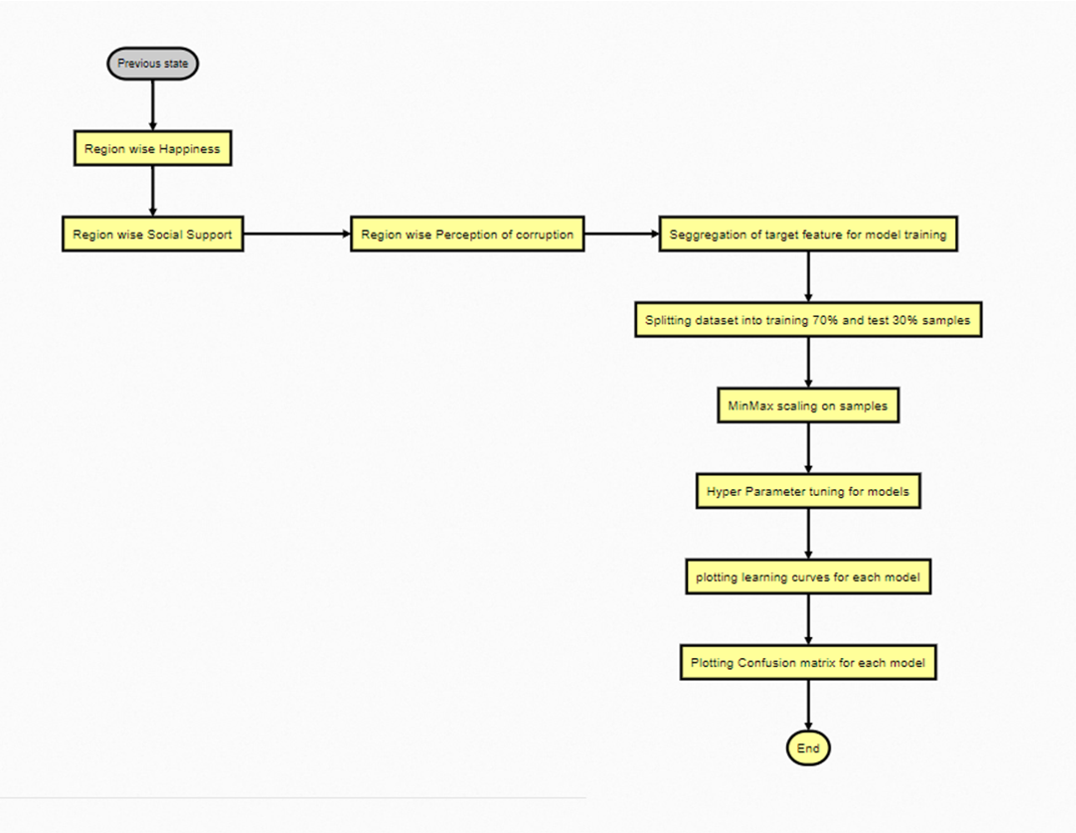
\includegraphics[width=15cm,height=15cm,keepaspectratio]{img/CodeFlow5.png}
    \caption{Code Flow diagram part 5}
    \label{fig:CodeFlow5}
\end{figure}

\end{enumerate}
\chapter{Results}
In this chapter, we attempt to present the outcomes of the five classification machine learning models covered in the preceding chapter using measures already discussed in the previous Chapter. 
\begin{scriptsize}
\begin{table}[h]
\begin{center}
\caption{Result of Evaluation Metrics on machine learning models.}
\label{tab: Evaluation Metrics}
\begin{tabular}{ | c | c | c |  c | c | c |}
\hline
Metric & Logistic Regression & Decision Tree & Random Forest & SVM & KNN\\
\hline
Accuracy  & 0.89 & 0.87 & 0.91 & 0.89 &	0.91\\
\hline
 Precision &  0.8689 &  0.8643 & 0.9058 & 0.8807 & 0.8965 \\
      \hline 	
Recall &  0.9169 &  0.8614 & 0.9130 & 0.9051 & 0.9249\\
    \hline
 F1 Score&  0.8923 &  0.8727 & 0.9094 & 0.8927 & 0.9105\\
    \hline
AUC Score&  0.8890 &  0.8712 & 0.9089 & 0.8910 & 0.9088\\
    \hline
    \end{tabular}
  \end{center}

\end{table}
\end{scriptsize}

\section{Logistic Regression}
It is one of the basic but very important classification models. We also chose this method and trained it on our dataset. The result shows that during training the model achieved an accuracy of 90\% while the accuracy was reduced to 89\% on the test sample as shown in Table \ref{tab: Evaluation Metrics} and logistic regression learning curve Figure \ref{fig: LR-LC}.
\begin{figure}
     \centering
     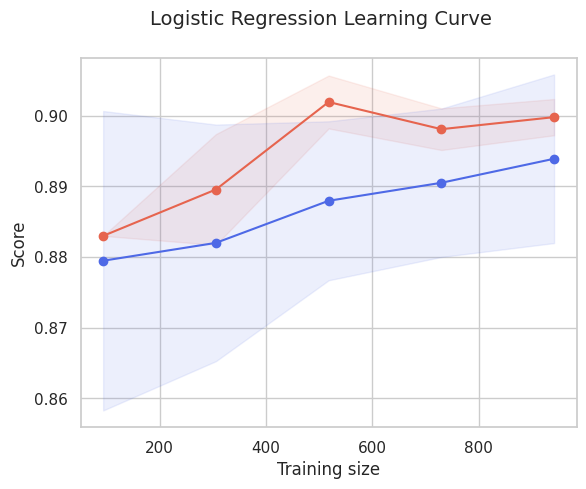
\includegraphics[width=15cm, height=12cm, keepaspectratio]{img/LR-LC.png}       \caption{Learning Curves for the logistic regression model.}                  
        \label{fig: LR-LC}
\end{figure}
\begin{figure}
    \centering
    
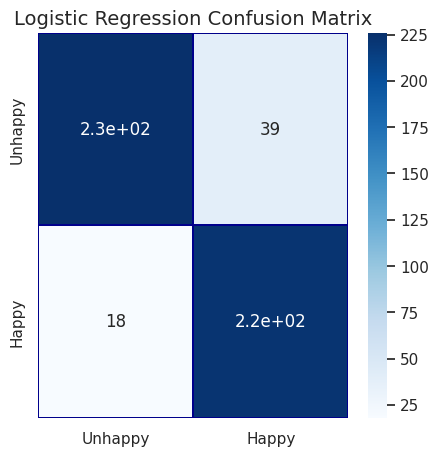
\includegraphics[width=15cm, height=12cm, keepaspectratio]{img/LR-CM.png}       \caption{Confusion Matrix for the logistic regression model.}                  
        \label{fig: LR-CM}
\end{figure}
\newpage


\section{Decision Tree}
The result shows that the decision tree classifier achieved an accuracy of 90\% during training the model. However, the accuracy of the model was reduced to 87\% on the test sample as shown in table \ref{tab: Evaluation Metrics}. The decision tree learning curve Figure \ref{fig: DT-LC} also second our observations mentioned.
\begin{figure}
\centering
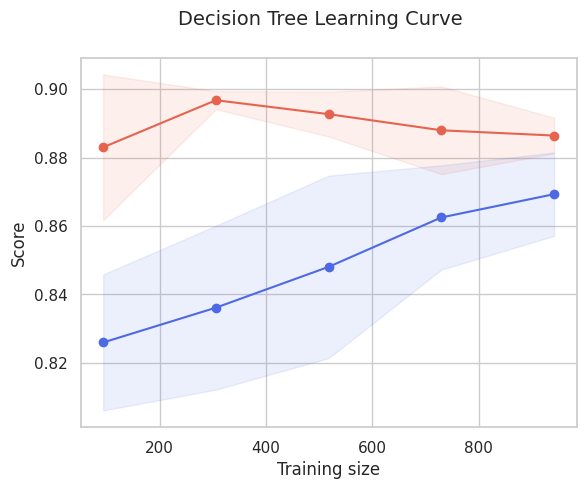
\includegraphics[width=15cm, height=12cm, keepaspectratio]{img/DT-LC.png}       \caption{Learning Curves for decision tree model.}                  
\label{fig: DT-LC}
\end{figure}
\begin{figure}
\centering
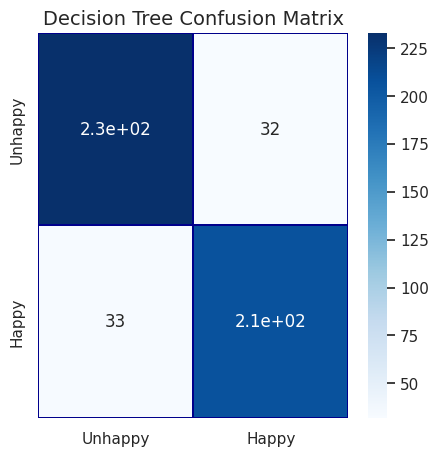
\includegraphics[width=15cm, height=12cm, keepaspectratio]{img/DT-CM.png}       \caption{Confusion Matrix for the result of decision tree model.}                  
\label{fig: DT-CM}
\end{figure}
\newpage
\section{Random Forest}
Random forest is an important classification model in resolving the classification problem. We applied this method to our dataset and during the training of the model. We achieved an accuracy of 99\% while the same was reduced to 91\% on the test sample as shown in Table \ref{tab: Evaluation Metrics}  and random forest learning curve Figure \ref{fig: RF-LC}.
\begin{figure}
\centering
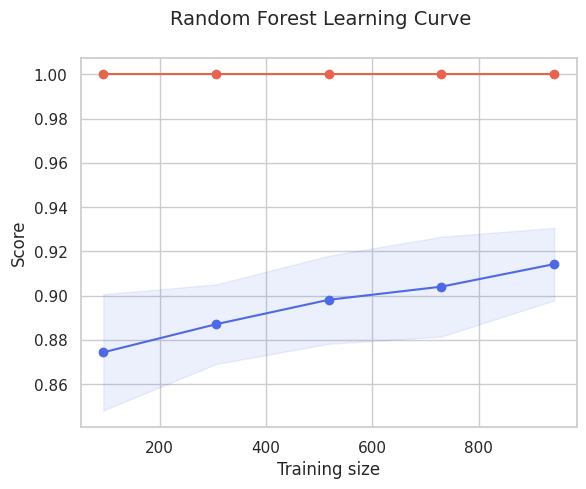
\includegraphics[width=15cm, height=12cm, keepaspectratio]{img/RF-LC.png}       
\caption{Learning Curves for random forest classification model.}                  
\label{fig: RF-LC}
\end{figure}
\begin{figure}
\centering
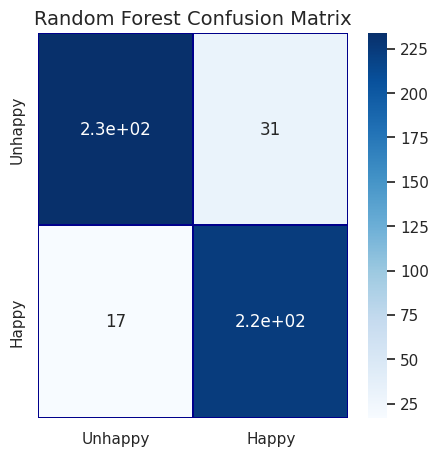
\includegraphics[width=15cm, height=12cm, keepaspectratio]{img/RF-CM.png}       
\caption{Confusion Matrix displaying the outcomes of random forest classification model.}                  
\label{fig: RF-CM}
\centering
\end{figure}
\newpage
\section{Support Vector Machine}
Another important classification model is known as support vector machine. SVM model shows an accuracy of 90\% on the training sample set while the accuracy was reduced to 89\% on the test sample as shown in support vector machine learning curve Figure \ref{fig: SVM-LC} and also in Table \ref{tab: Evaluation Metrics}.

\begin{figure}
     \centering
     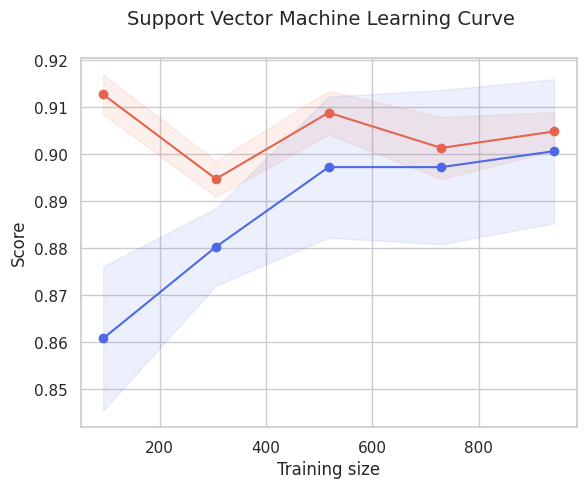
\includegraphics[width=15cm, height=12cm, keepaspectratio]{img/SVM-LC.png}       \caption{Learning Curve for support vector machine model.}                  
     \label{fig: SVM-LC}
\end{figure}
\begin{figure}
\centering
     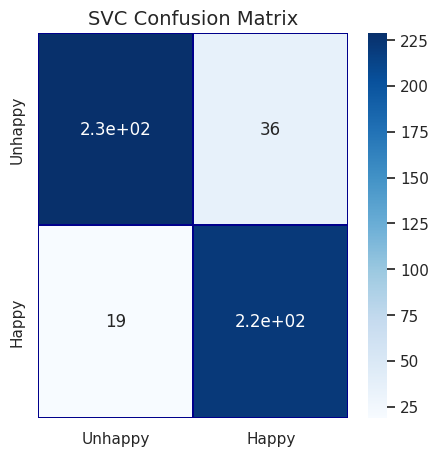
\includegraphics[width=15cm, height=12cm, keepaspectratio]{img/SVC-CM.png}       \caption{Confusion Matrix showing the result of  support vector machine model.}                  
     \label{fig: SVC-CM}
\end{figure}
\newpage
\section{K Nearest Neighbour}
During training the model KNN classifier achieved an accuracy of 90\%. Unprecedentedly, the accuracy of the KNN model was improved to 91\% for the test sample as shown in Table \ref{tab: Evaluation Metrics}  and its learning curve Figure \ref{fig: KNN-LC}.

\begin{figure}
\centering
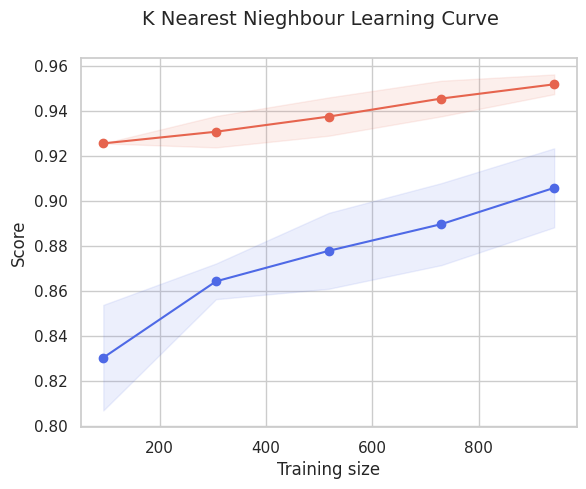
\includegraphics[width=15cm, height=12cm, keepaspectratio]{img/KNN-LC.png}       \caption{Learning Curves for KNN model.}                  
\label{fig: KNN-LC}
\end{figure}
\begin{figure}
\centering
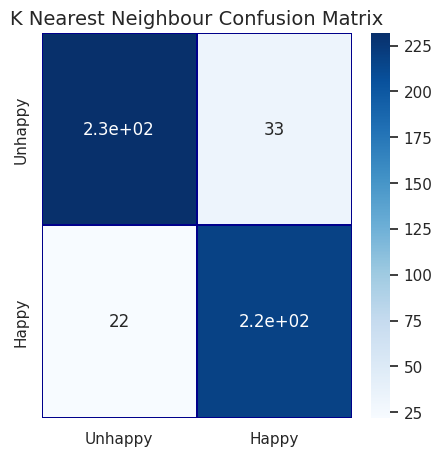
\includegraphics[width=15cm, height=10cm, keepaspectratio]{img/KNN-CM.png}       
\caption{Confusion Matrix showing the result of KNN model.}                  
\label{fig: KNN-CM}
\end{figure}
\newpage
\section{Future Work}
One area for future research could be exploring additional cultural factors that may impact happiness beyond what was examined in this thesis. For example, looking at how things like food, music, art, literature, and social norms in different cultures relate to happiness levels could provide new insights. Additional cultural dimensions like individualism vs. collectivism, or uncertainty avoidance could also be incorporated into the machine learning models to see if they improve predictive accuracy. Expanding the cultural factors considered could reveal new relationships and opportunities to improve understanding of cultural influences on happiness.

Another potential direction would be applying more advanced machine learning techniques like neural networks or deep learning algorithms. The models used in this thesis such as random forests and SVMs could be replaced or augmented with deep learning approaches which may better capture complex nonlinear relationships in the data. Tuning hyperparameters and experimenting with different model architectures could lead to improved performance. Additionally, testing other happiness datasets or surveys as training data could be insightful. The use of more sophisticated and flexible machine learning approaches may reveal new patterns and improve cultural happiness.

An interesting area for future exploration would be incorporating UN financial data such as GDP per capita, health expenditures, and education spending along with World Happiness Report survey data into the machine learning models. Adding these supplemental economic and social investment metrics for each country could reveal new relationships between financial factors, cultural dimensions, and happiness. The machine learning algorithms may be able to discern more nuanced patterns in how financing in areas like health and education interacts with cultural variables to predict happiness across nations. Fine-tuning models with this financial data fused could produce more robust and accurate cultural happiness predictions.

Additionally, integrating other relevant socio-economic datasets such as unemployment rates, income inequality, political stability, and life expectancy could provide a more holistic set of input factors. Combining survey-based happiness data with real-world statistics related to quality of life and opportunity could give greater context. Machine learning on this multidimensional fused dataset may better capture the complex dynamics between financial resources, social issues, culture, and happiness across countries. Building ensembles with models trained on different combinations of data could also improve generalisation. Pursuing a more interdisciplinary big data approach could yield superior cultural happiness insights.

Finally, a promising area for future exploration is how the findings from this thesis could inform public policy decisions. The cultural factors found to be associated with happiness levels could guide governments in determining which cultural aspects to invest in, promote, and preserve. Research into the relationship between culture and happiness using machine learning has the potential for real-world application. Turning the analytical insights into action could lead to tailored cultural initiatives and programs aimed at improving societal happiness and well-being. Further study is needed to determine how to best translate the machine learning findings into effective policy and cultural change for the enhancement of happiness cross-nationally.

\chapter{Conclusion}\label{ch:5}
Happy life is the desire of every human being and it depends on various factors of life. World Happiness Report 2023 dataset targeted some important factors that contribute to and damage the happiness of human beings. The aim of our study is to find out the impact of cultural, social, and economic elements on happiness. The exploratory analysis shows that Denmark was the happiest country in year 2022 while Finland ranked first in 2021 and second in 2022. On the other hand War-torn country, Afghanistan was the lowest in the ranks with some African Nations. We also observed that the log GDP per capita and social support have a positive impact on happiness while the perception of corruption and confidence in government has a negative impact on happiness.

We created our target variable from the life ladder feature into two classes happy and unhappy based on the mean value of the life ladder. After that, we trained and tested five classifiers on the dataset and the result of each was discussed based on evaluation metrics. Based on the evaluation of five machine learning classifiers on the dataset, the Random Forest model delivers the best overall performance. The Random Forest achieves top results on several key metrics including accuracy (0.91), precision (0.9058), AUC score (0.9089), and a high F1 score (0.9094). This indicates the Random Forest model balances both precision and recall to effectively minimize classification errors.

The SVM and KNN models achieve comparable performance to the Random Forest on some metrics, however, the Random Forest shows greater consistency across the board. For example, the SVM has slightly higher recall but lower precision and accuracy than the Random Forest.

The Logistic Regression has the weakest performance with the lowest accuracy, precision, recall, and AUC. This implies that the dataset may have complex non-linear relationships between variables that linear models fail to capture adequately.

In conclusion, the Random Forest classifier is the recommended predictive model based on superior and balanced results on key classification metrics. The algorithm's ensemble approach appears effective for this problem. In future work, tuning the Random Forest hyperparameters could potentially improve performance further. Overall, the study demonstrates the effective application of machine learning to achieve high accuracy on this classification task.


   \phantomsection
    \addcontentsline{toc}{chapter}{References}

 \bibliographystyle{IEEEtranN}

    \bibliography{bibliography}

\appendix
\chapter{Project Code}
\begin{lstlisting}[language=Python, caption=Libraries, breaklines]
import numpy as mpy
import scipy
from scipy import stats
import pandas as Pandi
from sklearn.metrics import confusion_matrix as ConfMat,classification_report as ClassRpt
from sklearn.model_selection import cross_val_predict as CrValPred,train_test_split as TrTsSp,ShuffleSplit as ShSp,learning_curve as LerCur,cross_val_score as CrValSc
from sklearn.model_selection import GridSearchCV as GrSrchCv
from sklearn.tree import DecisionTreeClassifier as DecTrCl
from sklearn.preprocessing import MinMaxScaler as MinMaxSc
import matplotlib.pyplot as MatPlt
from sklearn.linear_model import LogisticRegression as LogiReg
import seaborn as SeaBor
from sklearn.ensemble import RandomForestClassifier as RandFor
from sklearn.svm import SVC as SuppVecMach
from sklearn.neighbors import KNeighborsClassifier as KNearNeigh
import plotly.express as PlotEx

df = Pandi.read_csv("/content/drive/MyDrive/Zaigham-Dissertation/Dataset/World Happiness Report.csv")
df.head(7)

df.dtypes

df.shape

df.columns

MatPlt.figure(figsize=(17, 8))
SeaBor.heatmap(df.isnull())

df.isna().sum()

df.columns

df_null= Pandi.DataFrame(df.isna().sum())
df_null.columns =[ 'Missing Value Count']
df_null['Feature Name']=df.columns
df_null

SeaBor.barplot(data=df_null,y="Feature Name",x="Missing Value Count",orient="h")

df = df.dropna()
df.isna().sum()

df.shape

df.duplicated().value_counts()

df['Regional Indicator'].value_counts()

df['Country Name'].value_counts()

fig, ax = MatPlt.subplots(figsize=(10, 5))
SeaBor.heatmap(df.corr(), annot = True,ax=ax )
MatPlt.title("Relationship Between Features ")
MatPlt.show()

"""The correlation map shows that "Log GDP per Capita", "Social Support","Healthy Life Expectancy at Birth","Freedom to make choices" and positive effect has postive relationship with "Life Ladder". However, the Perception of corruption is negatively related with a value of -0.42. Lets confirm this with T-Test Analysis:"""

df.describe()

x = scipy.stats.pearsonr(df['Life Ladder'],  df['Log GDP Per Capita'])
x

"""Our Pearson Correlation Hypothesis is as Follows:

Ho - Columns do not correlate

Ha - Columns do Correlate

With P-value being 0.0, we can Reject Null Hypothesis (Ho)
"""

x = scipy.stats.pearsonr(df['Life Ladder'],  df['Social Support'])
x

"""Our Pearson Correlation Hypothesis is as Follows:

Ho - Columns do not correlate

Ha - Columns do Correlate

With P-value is near to 0.0, we can Reject Null Hypothesis (Ho)
"""

x = scipy.stats.pearsonr(df['Life Ladder'],  df['Healthy Life Expectancy At Birth'])
x

"""Our Pearson Correlation Hypothesis is as Follows:

Ho - Columns do not correlate

Ha - Columns do Correlate

With P-value is almost zero, we can Reject Null Hypothesis (Ho)
"""

x = scipy.stats.pearsonr(df['Life Ladder'],  df['Freedom To Make Life Choices'])
x

"""Our Pearson Correlation Hypothesis is as Follows:

Ho - Columns do not correlate

Ha - Columns do Correlate

With P-value is almost zero, we can Reject Null Hypothesis (Ho)
"""

x = scipy.stats.pearsonr(df['Life Ladder'],  df['Perceptions Of Corruption'])
x

def buildTarget(value):
    if value <= 5.4:
        return 0
    if value > 5.4:
        return 1

def buildTargetCat(value):
    if value <= 5.4:
        return 'Unhappy'
    if value > 5.4:
        return 'Happy'
target = df['Life Ladder'].apply(buildTarget)
target_cat = df['Life Ladder'].apply(buildTargetCat)

df['target']=target
df['target_cat']=target_cat

SeaBor.countplot(x='target_cat',data=df,palette="coolwarm_r")
MatPlt.title('Happiness Distribution', fontsize=14)
MatPlt.show()

df['Life Ladder'].hist()

df.head(30)

df['Life Ladder'].describe()

df_2022_happiest = df.groupby('Country Name')['Life Ladder'].mean().round(2).nlargest(5).reset_index()
fig, ax = MatPlt.subplots(figsize=(10, 5))
SeaBor.set(style = 'whitegrid')
palette = SeaBor.color_palette("Blues",n_colors=5)
palette.reverse()
SeaBor.barplot(ax =ax,data = df_2022_happiest , x = df_2022_happiest['Life Ladder'], y = df_2022_happiest['Country Name'],palette = palette)
ax.set_title(' 5 Most Happiest Countries of 2022')
ax.bar_label(ax.containers[0])

df_2022_saddest = df.groupby('Country Name')[['Country Name','Life Ladder']].mean().sort_values('Life Ladder', ascending=True).round(2).head(5).reset_index()
fig, ax = MatPlt.subplots(figsize=(10, 5))
SeaBor.set(style = 'whitegrid')
palette = SeaBor.color_palette("YlOrBr",n_colors=5)
palette.reverse()
SeaBor.barplot(ax =ax,data = df_2022_saddest , x = df_2022_saddest['Life Ladder'], y = df_2022_saddest['Country Name'],palette = palette)
ax.set_title(' 5 Least Happiest Countries of 2022')
ax.bar_label(ax.containers[0])

ss_2022_desc = Pandi.DataFrame(df.groupby('Country Name')[['Country Name','Social Support']].mean().sort_values('Social Support', ascending=False).round(2).head(5))
fig = PlotEx.bar(ss_2022_desc, x = ss_2022_desc.index, y = 'Social Support',
            title = 'Top Social Countrier (2022)', template = 'seaborn', color = ss_2022_desc.index, text = 'Social Support')
fig.update_layout( font=dict( family="Arial Black", size=16 ), showlegend=False )
fig.show()

ss_2022_asc = Pandi.DataFrame(df.groupby('Country Name')[['Country Name','Social Support']].mean().sort_values('Social Support', ascending=True).round(2).head(5))
fig = PlotEx.bar(ss_2022_asc, x = ss_2022_asc.index, y = 'Social Support',
            title = 'Lowest Social Countires (2022)', template = 'seaborn', color = ss_2022_asc.index, text = 'Social Support')
fig.update_layout( font=dict( family="Arial Black", size=16 ), showlegend=False )
fig.show()

cor_2022_desc = Pandi.DataFrame(df.groupby('Country Name')[['Country Name','Perceptions Of Corruption']].mean().sort_values('Perceptions Of Corruption', ascending=False).round(2).head(5))
fig = PlotEx.bar(cor_2022_desc, x = cor_2022_desc.index, y = 'Perceptions Of Corruption',
            title = 'Top 5 Most Corrupt Countires (2022)', template = 'seaborn', color = cor_2022_desc.index, text = 'Perceptions Of Corruption')
fig.update_layout( font=dict( family="Arial Black", size=16 ), showlegend=False )
fig.show()

cor_2022_asc = Pandi.DataFrame(df.groupby('Country Name')[['Country Name','Perceptions Of Corruption']].mean().sort_values('Perceptions Of Corruption', ascending=True).round(2).head(5))
fig = PlotEx.bar(cor_2022_asc, x = cor_2022_asc.index, y = 'Perceptions Of Corruption',
            title = 'Least Corrupt Countries (2022)', template = 'seaborn', color = cor_2022_asc.index, text = 'Perceptions Of Corruption')
fig.update_layout( font=dict( family="Arial Black", size=16 ), showlegend=False )
fig.show()

fig = PlotEx.choropleth(df, locations='Country Name', locationmode='country names',scope='world',color='Perceptions Of Corruption', color_continuous_scale= 'Viridis_r')
fig.update_layout(legend=dict(orientation="h"),
                  margin={'r':0,'t':0,'l':0,'b':0},
                  font=dict( family="Arial Black", size=14 ),
                  coloraxis_colorbar=dict(title = 'Corruption(2022)', ticks = 'outside', tickvals = [0,0.2,0.4,0.6,0.8,1.0], dtick = 7)
                  )
fig.show()

fig = PlotEx.choropleth(df, locations='Country Name', locationmode='country names',scope='world',color='Log GDP Per Capita', color_continuous_scale= 'Viridis_r')
fig.update_layout(legend=dict(orientation="h"),
                  margin={'r':0,'t':0,'l':0,'b':0},
                  font=dict( family="Arial Black", size=14 ),
                  coloraxis_colorbar=dict(title = 'Log GDP Per Capita (2022)', ticks = 'outside', tickvals = [6,8,10,12], dtick = 5)
                  )
fig.show()

fig = PlotEx.choropleth(df, locations='Country Name', locationmode='country names',scope='world',color='Social Support', color_continuous_scale= 'Viridis_r')
fig.update_layout(legend=dict(orientation="h"),
                  margin={'r':0,'t':0,'l':0,'b':0},
                  font=dict( family="Arial Black", size=14 ),
                  coloraxis_colorbar=dict(title = 'Social Supp (2022)', ticks = 'outside', tickvals = [0,0.2,0.4,0.6,0.8,1.0], dtick = 7)
                  )
fig.show()

fig = PlotEx.choropleth(df, locations='Country Name', locationmode='country names',scope='world',color='Social Support', color_continuous_scale= 'Viridis_r')
fig.update_layout(title = "Happines Comparison by Countries")
fig.update_layout(legend=dict(orientation="h"),
                  margin={'r':0,'t':0,'l':0,'b':0},
                  font=dict( family="Arial Black", size=14 ),
                  coloraxis_colorbar=dict(title = 'Life Ladder (2022)', ticks = 'outside', tickvals = [2,4,6,8], dtick = 4)
                  )
fig.show()

reg_ind_2022 = Pandi.DataFrame(df.groupby('Regional Indicator')[['Regional Indicator','Life Ladder']].mean().sort_values('Life Ladder', ascending=False).round(2).head(10))
fig = PlotEx.bar(reg_ind_2022, x = reg_ind_2022.index, y = 'Life Ladder',
            title = 'Happiness according to Regional Indicator - 2022', template = 'seaborn', color = reg_ind_2022.index, text = 'Life Ladder')
fig.update_layout( font=dict( family="Arial Black", size=16 ), showlegend=False )
fig.show()

reg_ind_2022 = Pandi.DataFrame(df.groupby('Regional Indicator')[['Regional Indicator','Social Support']].mean().sort_values('Social Support', ascending=False).round(2).head(10))
fig = PlotEx.bar(reg_ind_2022, x = reg_ind_2022.index, y = 'Social Support',
            title = 'Social Support according to Regional Indicator - 2022', template = 'seaborn', color = reg_ind_2022.index, text = 'Social Support')
fig.update_layout( font=dict( family="Arial Black", size=16 ), showlegend=False )
fig.show()

reg_ind_2022 = Pandi.DataFrame(df.groupby('Regional Indicator')[['Regional Indicator','Perceptions Of Corruption']].mean().sort_values('Perceptions Of Corruption', ascending=False).round(2).head(10))
fig = PlotEx.bar(reg_ind_2022, x = reg_ind_2022.index, y = 'Perceptions Of Corruption',
            title = 'Perceptions Of Corruption according to Regional Indicator - 2022', template = 'seaborn', color = reg_ind_2022.index, text = 'Perceptions Of Corruption')
fig.update_layout( font=dict( family="Arial Black", size=16 ), showlegend=False )
fig.show()

df.drop(['Country Name', 'Regional Indicator', 'Life Ladder','target_cat','target'], axis=1, inplace=True)

x_trn, x_valid, y_trn, y_valid = TrTsSp(df, target, test_size=.3)

print(f'x_trn: {x_trn.shape}, y_trn: {y_trn.shape}')
print(f'x_valid: {x_valid.shape}, y_valid: {y_valid.shape}')

scaler = MinMaxSc()

x_trn_scaled = scaler.fit_transform(x_trn)
x_valid_scaled = scaler.transform(x_valid)

modelLR=LogiReg()
CrValSc(modelLR, x_trn_scaled, y_trn, cv=5).mean().round(2)

modelRFC = RandFor(n_estimators=100, n_jobs=-1, random_state=23)
CrValSc(modelRFC, x_trn_scaled, y_trn, cv=5).mean().round(2)

modelSVC = SuppVecMach(kernel='rbf', C=1)
CrValSc(modelSVC, x_trn_scaled, y_trn, cv=5).mean().round(2)

modelKNN = KNearNeigh()
CrValSc(modelKNN, x_trn_scaled, y_trn, cv=5).mean().round(2)

modelDT = DecTrCl()
CrValSc(modelDT, x_trn_scaled, y_trn, cv=5).mean().round(2)

LR_params = {"penalty": ['l1', 'l2','elasticnet'], 'C': [ 0.01, 0.1, 1, 10, 100]}
grid_LR = GrSrchCv(LogiReg(), LR_params)
grid_LR.fit(x_trn_scaled, y_trn)
LR = grid_LR.best_estimator_
print("Logistic Regression:",LR)

KNN_params = {"n_neighbors": list(range(2,5,1)), 'algorithm': ['auto', 'ball_tree', 'kd_tree', 'brute']}

grid_KNN = GrSrchCv(KNearNeigh(), KNN_params)
grid_KNN.fit(x_trn_scaled, y_trn)
KNN = grid_KNN.best_estimator_
print("KNN:",KNN)

tree_params = {"criterion": ["gini", "entropy"], "max_depth": list(range(2,4,1)),
              "min_samples_leaf": list(range(5,7,1))}
grid_tree = GrSrchCv(DecTrCl(), tree_params)
grid_tree.fit(x_trn_scaled, y_trn)

DT = grid_tree.best_estimator_
print("Decision Tree:",DT)

rf_params = {"n_estimators"      : [10,20,30],
            "max_features"      : ["sqrt", "log2"],
            "min_samples_split" : [2,4,8],
            "bootstrap": [True, False]}
grid_rf = GrSrchCv(RandFor(), rf_params, n_jobs=-1, cv=5)
grid_rf.fit(x_trn_scaled, y_trn)

RF = grid_rf.best_estimator_
print("Random Forest:",RF)

SVC_params = {'C': [0.5, 0.7, 0.9, 1], 'kernel': ['rbf', 'poly', 'sigmoid', 'linear']}
grid_SVC = GrSrchCv(SuppVecMach(), SVC_params)
grid_SVC.fit(x_trn_scaled, y_trn)

SVC_best = grid_SVC.best_estimator_
print("Support Vector Machine:",SVC_best)

LR_score = CrValSc(LR, x_trn_scaled, y_trn, cv=5)
KNN_score = CrValSc(KNN, x_trn_scaled, y_trn, cv=5)
DT_score = CrValSc(DT, x_trn_scaled, y_trn, cv=5)
RF_score = CrValSc(RF, x_trn_scaled, y_trn, cv=5)
SVC_score = CrValSc(SVC_best, x_trn_scaled, y_trn, cv=5)

print('LR-:', round(LR_score.mean() * 100, 2), '%\n KNN-:', round(KNN_score.mean() * 100, 2), '%')
print('DT-:', round(DT_score.mean() * 100, 2), '% \n RF-:', round(RF_score.mean() * 100, 2), '%\n SVC-:', round(SVC_score.mean() * 100, 2), '%')

train_sizes, tr_rating, ts_rating = LerCur(LR, x_trn_scaled, y_trn, cv=None,n_jobs=1, train_sizes=mpy.linspace(.1, 1.0, 5))
tr_rating_mean = mpy.mean(tr_rating, axis=1)
tr_rating_std = mpy.std(tr_rating, axis=1)
ts_rating_mean = mpy.mean(ts_rating, axis=1)
ts_rating_std = mpy.std(ts_rating, axis=1)
MatPlt.fill_between(train_sizes, tr_rating_mean - tr_rating_std,
                  tr_rating_mean + tr_rating_std, alpha=0.1,
                  color="#E6644E")
MatPlt.fill_between(train_sizes, ts_rating_mean - ts_rating_std,
                  ts_rating_mean + ts_rating_std, alpha=0.1, color="#4E69E6")
MatPlt.plot(train_sizes, tr_rating_mean, 'o-', color="#E6644E",
          label="Training Rating")
MatPlt.plot(train_sizes, ts_rating_mean, 'o-', color="#4E69E6",
          label="Cross validation RAting")
MatPlt.suptitle("Learning Curve \n Logistic Regression", fontsize=14)
MatPlt.xlabel('Training Sample size')
MatPlt.ylabel('Rating')

train_sizes, tr_rating, ts_rating = LerCur(DT, x_trn_scaled, y_trn, cv=None,n_jobs=1, train_sizes=mpy.linspace(.1, 1.0, 5))
tr_rating_mean = mpy.mean(tr_rating, axis=1)
tr_rating_std = mpy.std(tr_rating, axis=1)
ts_rating_mean = mpy.mean(ts_rating, axis=1)
ts_rating_std = mpy.std(ts_rating, axis=1)
MatPlt.fill_between(train_sizes, tr_rating_mean - tr_rating_std,
                  tr_rating_mean + tr_rating_std, alpha=0.1,
                  color="#E6644E")
MatPlt.fill_between(train_sizes, ts_rating_mean - ts_rating_std,
                  ts_rating_mean + ts_rating_std, alpha=0.1, color="#4E69E6")
MatPlt.plot(train_sizes, tr_rating_mean, 'o-', color="#E6644E",
          label="Training score")
MatPlt.plot(train_sizes, ts_rating_mean, 'o-', color="#4E69E6",
          label="Cross-validation score")
MatPlt.suptitle("Learning Curve \n Decision Tree ", fontsize=14)
MatPlt.xlabel('Training size')
MatPlt.ylabel('Score')

train_sizes, tr_rating, ts_rating = LerCur(RF, x_trn_scaled, y_trn, cv=None,n_jobs=1, train_sizes=mpy.linspace(.1, 1.0, 5))
tr_rating_mean = mpy.mean(tr_rating, axis=1)
tr_rating_std = mpy.std(tr_rating, axis=1)
ts_rating_mean = mpy.mean(ts_rating, axis=1)
ts_rating_std = mpy.std(ts_rating, axis=1)
MatPlt.fill_between(train_sizes, tr_rating_mean - tr_rating_std,
                  tr_rating_mean + tr_rating_std, alpha=0.1,
                  color="#E6644E")
MatPlt.fill_between(train_sizes, ts_rating_mean - ts_rating_std,
                  ts_rating_mean + ts_rating_std, alpha=0.1, color="#4E69E6")
MatPlt.plot(train_sizes, tr_rating_mean, 'o-', color="#E6644E",
          label="Training score")
MatPlt.plot(train_sizes, ts_rating_mean, 'o-', color="#4E69E6",
          label="Cross-validation score")
MatPlt.suptitle("Learning Curve \n Random Forest", fontsize=14)
MatPlt.xlabel('Training size')
MatPlt.ylabel('Score')

train_sizes, tr_rating, ts_rating = LerCur(SVC_best, x_trn_scaled, y_trn, cv=None,n_jobs=1, train_sizes=mpy.linspace(.1, 1.0, 5))
tr_rating_mean = mpy.mean(tr_rating, axis=1)
tr_rating_std = mpy.std(tr_rating, axis=1)
ts_rating_mean = mpy.mean(ts_rating, axis=1)
ts_rating_std = mpy.std(ts_rating, axis=1)
MatPlt.fill_between(train_sizes, tr_rating_mean - tr_rating_std,
                  tr_rating_mean + tr_rating_std, alpha=0.1,
                  color="#E6644E")
MatPlt.fill_between(train_sizes, ts_rating_mean - ts_rating_std,
                  ts_rating_mean + ts_rating_std, alpha=0.1, color="#4E69E6")
MatPlt.plot(train_sizes, tr_rating_mean, 'o-', color="#E6644E",
          label="Training score")
MatPlt.plot(train_sizes, ts_rating_mean, 'o-', color="#4E69E6",
          label="CV  Score")
MatPlt.suptitle("Learning Curve \n Support Vector Machine ", fontsize=14)
MatPlt.xlabel('Training size')
MatPlt.ylabel('Score')

train_sizes, tr_rating, ts_rating = LerCur(KNN, x_trn_scaled, y_trn, cv=None,n_jobs=1, train_sizes=mpy.linspace(.1, 1.0, 5))
tr_rating_mean = mpy.mean(tr_rating, axis=1)
tr_rating_std = mpy.std(tr_rating, axis=1)
ts_rating_mean = mpy.mean(ts_rating, axis=1)
ts_rating_std = mpy.std(ts_rating, axis=1)
MatPlt.fill_between(train_sizes, tr_rating_mean - tr_rating_std,
                  tr_rating_mean + tr_rating_std, alpha=0.1,
                  color="#E6644E")
MatPlt.fill_between(train_sizes, ts_rating_mean - ts_rating_std,
                  ts_rating_mean + ts_rating_std, alpha=0.1, color="#4E69E6")
MatPlt.plot(train_sizes, tr_rating_mean, 'o-', color="#E6644E",
          label="Training score")
MatPlt.plot(train_sizes, ts_rating_mean, 'o-', color="#4E69E6",
          label="CV score")
MatPlt.suptitle("Learning Curve \n K Nearest Nieghbour ", fontsize=14)
MatPlt.xlabel('Training size')
MatPlt.ylabel('Score')

LR_pred = CrValPred(LR, x_trn_scaled, y_trn, cv=5,
                             method="decision_function")

KNN_pred = CrValPred(KNN, x_trn_scaled, y_trn, cv=5)

SVC_pred = CrValPred(SVC_best, x_trn_scaled, y_trn, cv=5,
                             method="decision_function")

DT_pred = CrValPred(DT, x_trn_scaled, y_trn, cv=5)

RF_pred = CrValPred(RF, x_trn_scaled, y_trn, cv=5)

print("Logistic Regresssion has a accuracy score of ", round(LR_pred.mean(), 2) * 100, "%")
print("KNN has a accuracy score of", round(KNN_pred.mean(), 2) * 100, "%")
print("SVC has a accuracy score of", round(SVC_pred.mean(), 2) * 100, "%")
print("DT has a accuracy score of", round(DT_pred.mean(), 2) * 100, "%")
print("RF has a accuracy score of", round(RF_pred.mean(), 2) * 100, "%")

LR.fit(x_trn_scaled, y_trn)
y_pred_LR = LR.predict(x_valid_scaled)
LR_cf = ConfMat(y_valid, y_pred_LR )
fig, (ax1) = MatPlt.subplots(ncols=1, figsize=(5,5))
SeaBor.heatmap(LR_cf,
            xticklabels=['Unhappy', 'Happy'],
            yticklabels=['Unhappy', 'Happy'],
            annot=True,ax=ax1,
            linewidths=.2,linecolor="Darkblue", cmap="Blues")
MatPlt.title('Confusion Matrix', fontsize=14)
MatPlt.show()

KNN.fit(x_trn_scaled, y_trn)
y_pred_KNN = KNN.predict(x_valid_scaled)
KNN_cf = ConfMat(y_valid, y_pred_LR )
fig, (ax1) = MatPlt.subplots(ncols=1, figsize=(5,5))
SeaBor.heatmap(KNN_cf,
            xticklabels=['Unhappy', 'Happy'],
            yticklabels=['Unhappy', 'Happy'],
            annot=True,ax=ax1,
            linewidths=.2,linecolor="Darkblue", cmap="Blues")
MatPlt.title('Confusion Matrix', fontsize=14)
MatPlt.show()

RF.fit(x_trn_scaled, y_trn)
y_pred_RF = RF.predict(x_valid_scaled)
RF_cf = ConfMat(y_valid, y_pred_RF )
print('Confusion Matrix\n')
print(RF_cf)
SeaBor.heatmap(RF_cf, annot=True, cmap="Blues")

DT.fit(x_trn_scaled, y_trn)
y_pred_DT = DT.predict(x_valid_scaled)
DT_cf = ConfMat(y_valid, y_pred_DT )
print('Confusion Matrix\n')
print(DT_cf)
SeaBor.heatmap(DT_cf, annot=True, cmap="Blues")

SVC_best.fit(x_trn_scaled, y_trn)
y_pred_SVC = SVC_best.predict(x_valid_scaled)
SVC_cf = ConfMat(y_valid, y_pred_SVC )
print('Confusion Matrix\n')
print(SVC_cf)
SeaBor.heatmap(SVC_cf, annot=True, cmap="Blues")

print('\nClassification Report\n')
print(ClassRpt(y_valid, y_pred_LR, target_names=['Unhappy', 'Happy']))
\end{lstlisting}

\end{document}

